\part{Capítulo once}
\graphicspath{ {11_Capitulo/img/exportados/}, {W_Varios/2_Portada_capitulos/} }

%----------------------------------------------------------------------------------------
%	CHAPTER 11
%----------------------------------------------------------------------------------------

\chapterimage{ima2} % Chapter heading image

\chapter{Tasa interna de retorno TIR}

\section{Mapa Mental}
\begin{center}
	% 	tamaño maximo de imagenes, una cuartilla, aprox: 13,97 cm X 20,00
	% cm, mínimo: 10.5 x 16.4 cm
	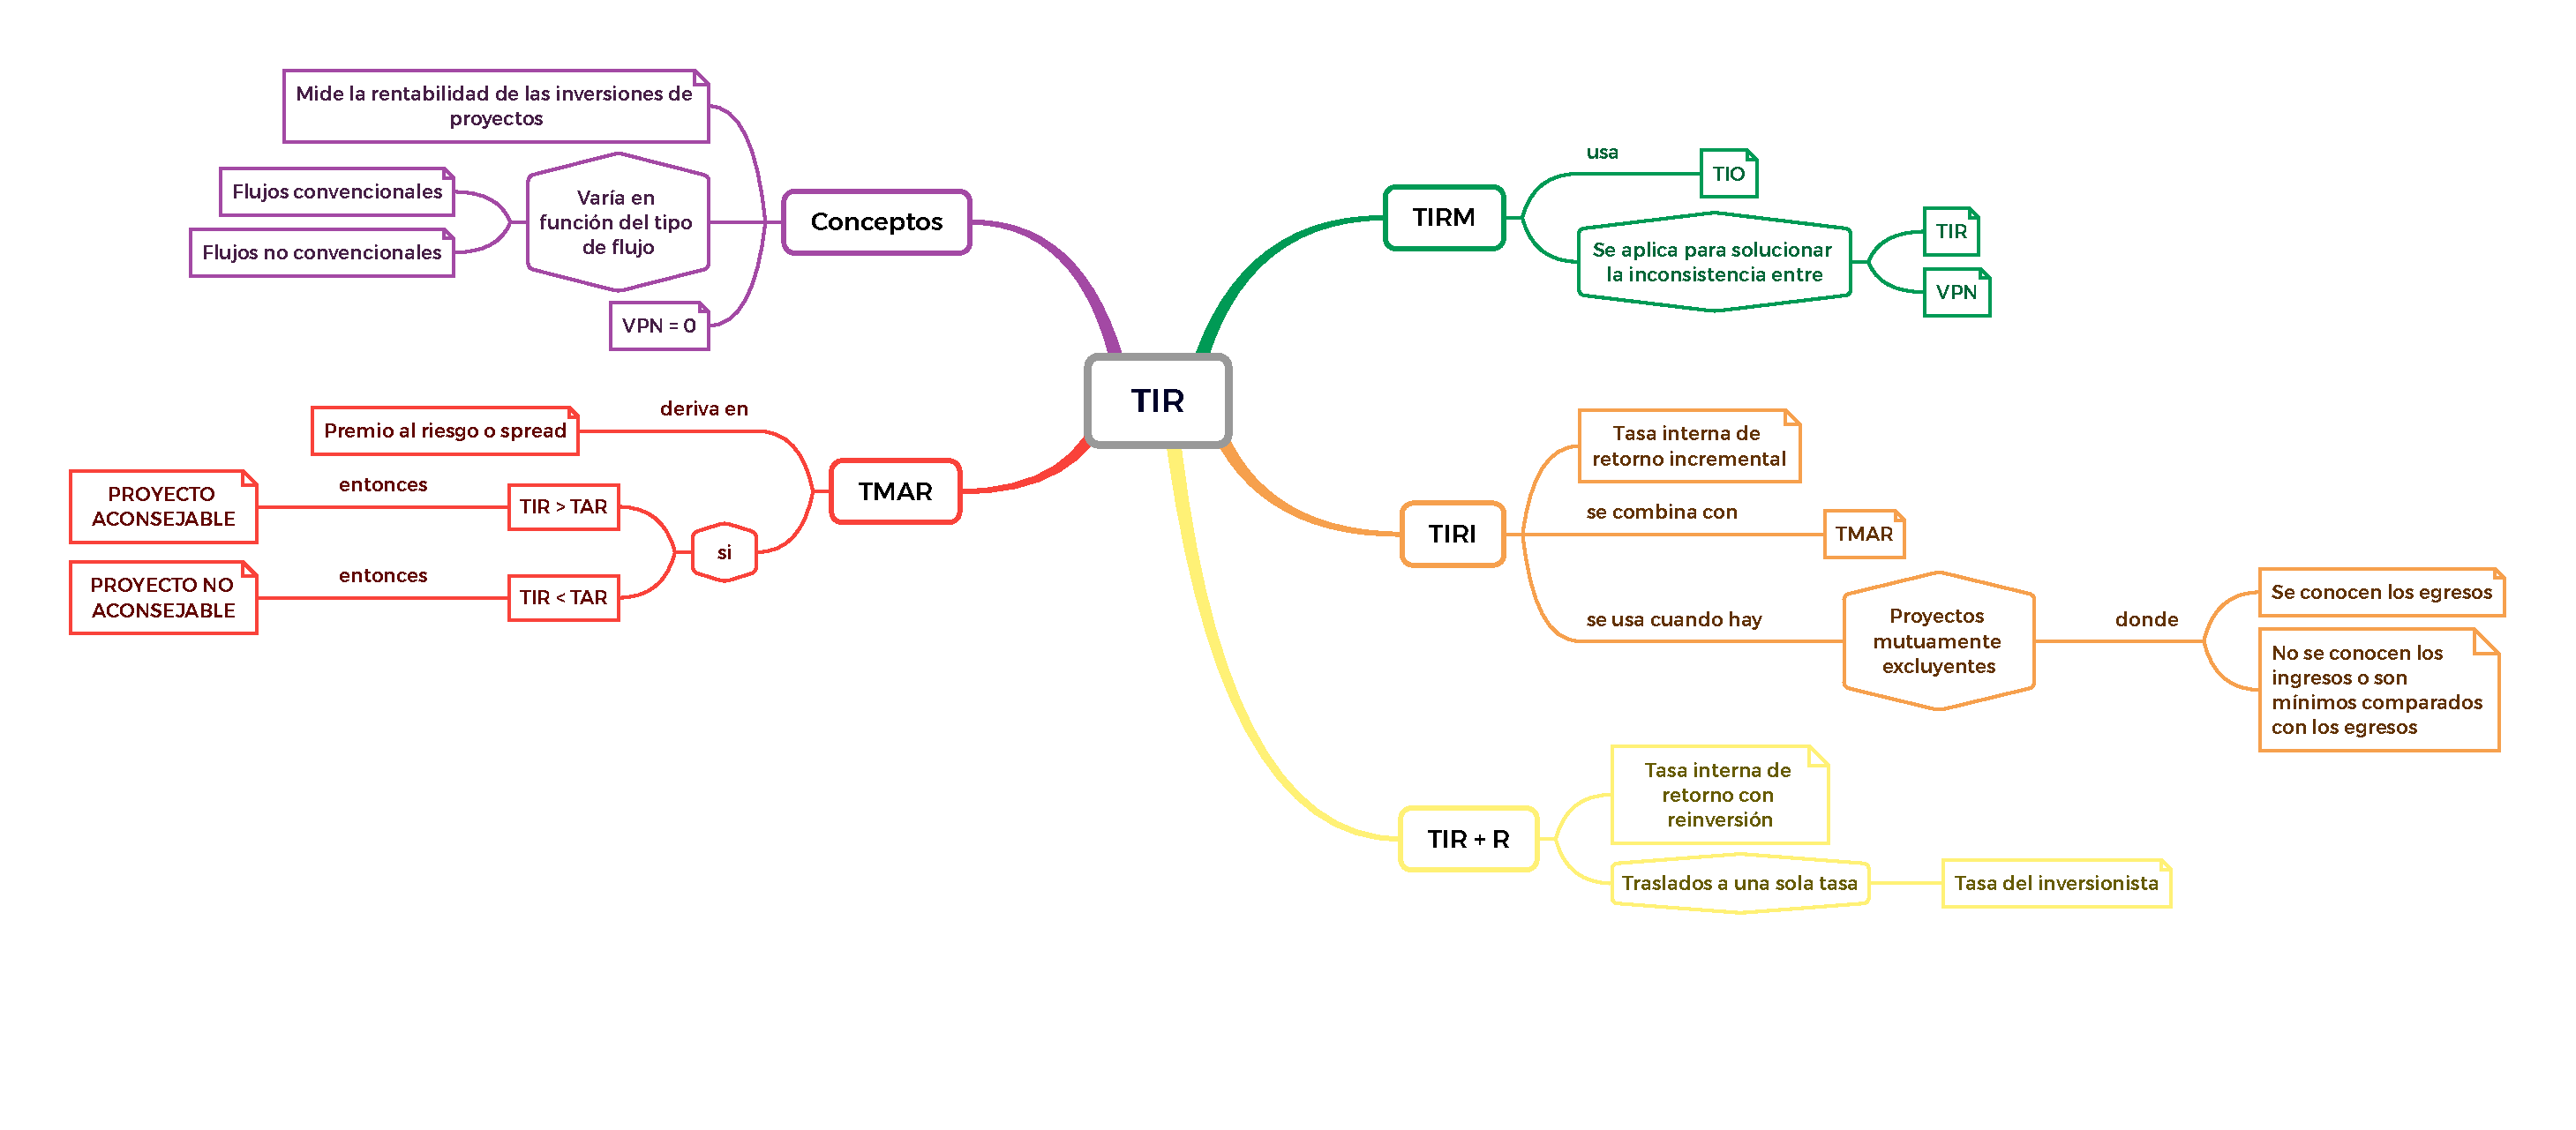
\includegraphics[height=5.65cm]{explicacion/mapamentalCap11.pdf}
\end{center}

%----------------------------------
%Tabla de fórmulas
%------------------------------------------

\newpage
\section{{Fórmulas del capítulo}}
\vspace{\baselineskip}
\begin{spacing}{1}
	\begin{center}
		\begin{tabular}{ |p{4.5cm}|p{4.5cm}| p{4.5cm}|}
			\hline
			\rowcolor[HTML]{FFB183}
			\begin{center}\textbf{\fontsize{9}{11}Fórmula} \end{center} & \begin{center} \textbf{\fontsize{9}{11}Nombre} \end{center} & \begin{center} \textbf{\fontsize{9}{11}Excel} \end{center} \\ \hline
			\text{\fontsize{9}{11}F = $P(1+i)^n$}
			                                                                 & Valor futuro                                                     & VF(i;n;;VA,0)                                                   \\ \hline

			j = im                                                           & Tasa nominal anual vencida                                              & TASA.NOMINAL(i;m)                                               \\ \hline

			P = $\frac{F}{(1 + i)^{n}}$                                      & Valor presente                                                   & VA(i;n;;VF,0)                                                   \\ \hline

			${(1 + i_{1})^{m_{1}}}$ = ${(1 + i_{2})^{m_{2}}}$                & Equivalencia de tasas periódicas                                         & TASA(m;;-1;1+i)                                                 \\ \hline

			VPN =	$\sum F_{n}(1+i)^{-n}$ \                                   & Valor Presente Neto                                              & -                                                               \\ \hline
		\end{tabular}
	\end{center}
\end{spacing}


\section{Introducción}
La tasa interna de retorno (TIR) es uno de los índices más aceptados por el público, porque mide la rentabilidad de una inversión. Sin embargo, para los especialistas no tiene la misma aceptación porque se presta a errores. %% L: Revisar expresión
En algunas ocasiones, la decisión que se toma con el VPN no coincide con la decisión que se toma con la TIR. Esto ocurre ya que la TIR no se aplica correctamente y en tales casos, es necesario utilizar otra técnica para lograr que los resultados obtenidos con la TIR coincidan con los resultados que se obtengan con el VPN.

Financieramente, la TIR es la tasa a la cual los flujos de caja son descontados de forma tal que los ingresos y los egresos sean iguales; desde el punto de vista matemático, la TIR es la tasa a la cual el VPN se hace cero.\\[0.3mm]

Existen dos clases de flujos de caja: los flujos convencionales y los flujos no convencionales.\\

\textbf{Los flujos convencionales} son aquellos donde primero aparecen los egresos y después aparecen los ingresos o viceversa.\vspace{0.2cm}

\textbf{Los flujos no convencionales} son aquellos donde figuran intercalados los ingresos y los egresos.
\\
Ejemplos de flujos de caja \\

\textbf{Figura 1} \\
\textit{Flujo convencional}
\begin{center}
	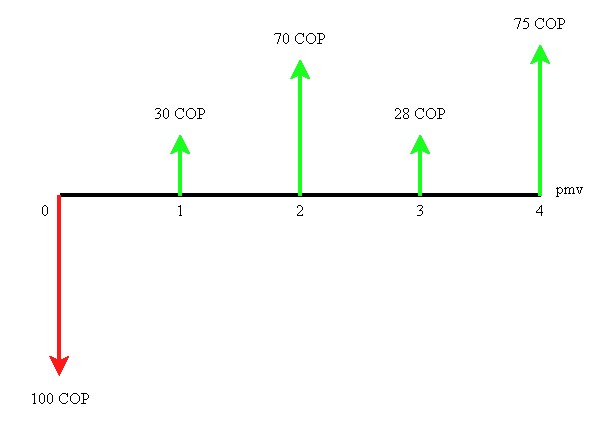
\includegraphics[scale=1]{explicacion/Graf1Cap11.pdf}
\end{center}
\text{}\\\\
\textbf{Figura 2} \\
\textit{Flujo no convencional}
\begin{center}
	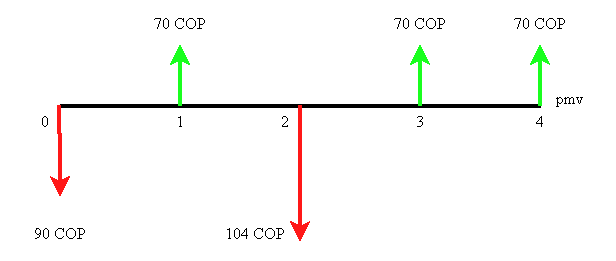
\includegraphics[scale=1]{explicacion/Graf2Cap11.pdf}
\end{center}

El procedimiento que se usa para calcular la TIR varía dependiendo del número de alternativas a analizar y de la forma en que se encuentren distribuidos los ingresos y los egresos a lo largo del horizonte de planificación; veamos algunos ejemplos: \\

\textbf{Ejemplo 1}\\

Una persona está pensando en construir un parqueadero, para tal fin, toma en alquiler un lote por un plazo de 5 años. El costo de la construcción, incluidos los impuestos y las licencias, es de 15.000.000 COP; se estima que los ingresos después de descontar el valor de los arriendos e impuestos, es decir, los ingresos netos, serán 5.000.000 COP, los cuales crecerán cada año aproximadamente de acuerdo al índice de inflación que se estima en un 20\% período anual vencido. Si el inversionista gana normalmente en todos sus negocios un 35\% período anual vencido. ¿Es aconsejable este negocio?
\\

\textbf{Solución.}\\
\begin{center}
    \renewcommand{\arraystretch}{1.5} %Margenes de las celdas
    \begin{longtable}{|c|c|c|} %Creacion de una cuadricula de 4 columnas
        \hline % Crea una linea horizonal arriba
        \rowcolor[HTML]{FFB183} %Define el color de la primera fila
        %%% INICIO ASIGNACION PERIODO FOCAL %%%%
        %%%INICIO TITULO
        %MEZCLAR 3 COLUMNAS EN UNA SOLA
        \multicolumn{3}{|c|}{\cellcolor[HTML]{FFB183}\textbf{1. Asignación periodo focal}}                                                                                                                                            \\ \hline
        %%FIN TITULO
        \multicolumn{3}{|c|}{$pf : 0 pav$}                                                                                                                                                                                            \\
        %%%FIN ASIGNACION PERIODO FOCAL
        \hline
        %%%% INICIO DECLARACION DE VARIABLES
        %%%INICIO TITULO
        \multicolumn{3}{|c|}{\cellcolor[HTML]{FFB183}\textbf{2. Declaración de variables}}                                                                                                                                            \\ \hline
        \multicolumn{1}{|c|}{\cellcolor[HTML]{FFB183}\textbf{Valores monetarios}}    & \multicolumn{1}{c|}{\cellcolor[HTML]{FFB183}\textbf{Valores no monetarios}} & \multicolumn{1}{c|}{\cellcolor[HTML]{FFB183}\textbf{Incógnitas}} \\ \hline
        %%%FIN TITULO
        %Cada & hace referencia al paso de la siguiente columna
        %Cada \\ hace referencia a un salto de linea
        $\textbf{Inversión inicial} = $ $15\text{.}000\text{.}000 \text{ COP}$       & $i_{1} = 20\% pav$                                                          &                                                                  \\
        $\textbf{Ingresos netos primer año} =$ $5\text{.}000\text{.}000 \text{ COP}$ & $i_{2} = TIO = 35\% pav$                                                    & $i = TIR = ?\% pav$                                              \\
                                                                                     & $n = 5 pav$                                                                 &                                                                  \\

        \hline
        %%% FIN DECLARACION DE VARIABLES
        %%%INICIO DIAGRAMA DE FLUJO
        %%INICIO TITULO
        \multicolumn{3}{|c|}{\cellcolor[HTML]{FFB183}\textbf{3. Diagrama de flujo de caja}}                                                                                                                                           \\ \hline
        %%FIN TITULO
        %%%%%%%%%%%%% INSERCIÓN DE LA IMAGEN
        %Mezclamos 3 columnas y pondremos el dibujo
        %Deberán descargar las imágenes respectivas del drive y pegarlas en la carpeta
        %n_capitulo/img/ejemplos/1/capitulo1ejemplo1.pdf  (el /1/ es el numero del ejemplo)
        \multicolumn{3}{|c|}{ 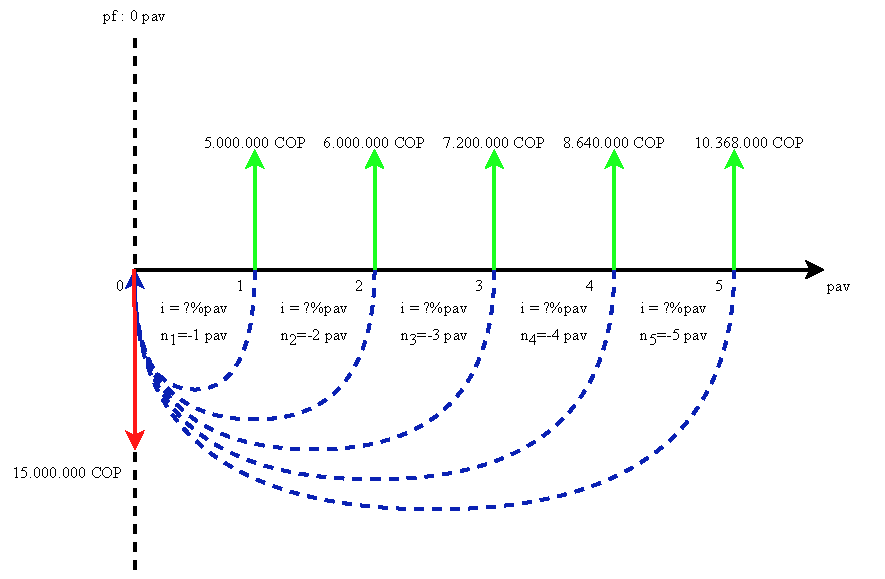
\includegraphics[scale=0.9]{ejemplos/1/Graf1Ej1Cap11.pdf} }
        \\ \hline
        %%%%%%%%%%%%% FIN INSERCIÓN DE IMAGEN
        %%%FIN DIAGRAMA DE FLUJO
        %%%INICIO DECLARACION DE FORMULAS
        %%INICIO TITULO
        \multicolumn{3}{|c|}{\cellcolor[HTML]{FFB183}\textbf{4. Declaración de fórmulas}}                                                                                                                                             \\ \hline
        %%FIN TITULO
        %%%%%%%%%%% INICIO MATEMÁTICAS
        \multicolumn{3}{|c|}{$F = P(1+i)^n \hspace{0.3cm} $ Valor futuro.}                                                                                                                                                     \\
        \multicolumn{3}{|c|}{$VPN =\sum F_{n}(1+i)^{-n} $ Valor presente neto.}                                                                                                                                                       \\ \hline
        %%%%%%%%%% FIN MATEMÁTICAS
        %%%FIN DECLARACION DE FORMULAS
        %%%INICIO DESARROLLO MATEMATICO
        %%INICIO TITULO
        \multicolumn{3}{|c|}{\cellcolor[HTML]{FFB183}\textbf{5. Desarrollo matemático}}                                                                                                                                               \\ \hline
        %%FIN TITULO
        %%%%%%%%%%% INICIO MATEMÁTICAS
        \multicolumn{3}{|c|}{$F_1 = $ $5\text{.}000\text{.}000 \text{ COP}$  $(1 + 0.2)^{1} = $ $6\text{.}000\text{.}000 \text{ COP}$ }                                                                                               \\
        \multicolumn{3}{|c|}{$F_2 = $ $6\text{.}000\text{.}000 \text{ COP}$  $(1 + 0.2)^{1} = $ $7\text{.}200\text{.}000 \text{ COP}$ }                                                                                               \\
        \multicolumn{3}{|c|}{$F_3 = $ $7\text{.}200\text{.}000 \text{ COP}$  $(1 + 0.2)^{1} = $ $8\text{.}640\text{.}000 \text{ COP}$ }                                                                                               \\
        \multicolumn{3}{|c|}{$F_4 = $ $8\text{.}640\text{.}000 \text{ COP}$  $(1 + 0.2)^{1} = $ $10\text{.}368\text{.}000 \text{ COP}$ }                                                                                              \\
        \multicolumn{3}{|c|}{ $ VPN = -15\text{ COP} + 5\text{ COP}(1+i)^{-1} + 6\text{ COP}(1+i)^{-2} + 7.2\text{ COP}(1+i)^{-3} +$  }                                                                                               \\
        \multicolumn{3}{|c|}{$ 8,64\text{ COP}(1+i)^{-4} + 10,368\text{ COP}(1+i)^{-5}$}                                                                                                                                              \\
        \multicolumn{3}{|c|}{$\textbf{La TIR la tasa en la cual el VPN se hace cero:}  $}                                                                                                                                             \\

        \multicolumn{3}{|c|}{$ VPN = -15\text{ COP} + 5\text{ COP}(1+i)^{-1} + 6\text{ COP}(1+i)^{-2} + 7.2\text{ COP}(1+i)^{-3}$}                                                                                                    \\
        \multicolumn{3}{|c|}{$8,64\text{ COP}(1+i)^{-4} + 10,368\text{ COP}(1+i)^{-5} = 0$}                                                                                                                                           \\

        \multicolumn{3}{|c|}{$\textbf{La solucion manual requiere usar la interpolación, para ello escogemos valores para i no }  $}                                                                                                  \\
        \multicolumn{3}{|c|}{$ \textbf{muy alejados entre sí de tal forma que la función sea una vez positiva y otra negativa, así:}$}                                                                                                \\
        \multicolumn{3}{|c|}{$ \textit{Primer ensayo: }$}                                                                                                                                                                             \\
        \multicolumn{3}{|c|}{$ \textit{i = 34\% pav}$}                                                                                                                                                                                \\
        \multicolumn{3}{|c|}{$ VPN = -15\text{ COP} + 5\text{ COP}(1+0.34)^{-1} + 6\text{ COP}(1+0.34)^{-2} + 7.2\text{ COP}(1+0.34)^{-3}$}                                                                                           \\
        \multicolumn{3}{|c|}{$+8,64COP(1+0.34)^{-4} + 10,368\text{ COP}(1+0.34)^{-5}=0.144763$}                                                                                                                                       \\
        \multicolumn{3}{|c|}{$ \textit{Segundo ensayo: }$}                                                                                                                                                                            \\
        \multicolumn{3}{|c|}{$ \textit{i = 35\% pav}$}                                                                                                                                                                                \\
        \multicolumn{3}{|c|}{$ VPN = -15\text{ COP} + 5\text{ COP}(1+0.35)^{-1} + 6\text{ COP}(1+0.35)^{-2} + 7.2\text{ COP}(1+0.35)^{-3} +$}                                                                                         \\
        \multicolumn{3}{|c|}{$8,64\text{ COP}(1+0.35)^{-4} + 10,368\text{ COP}(1+0.35)^{-5} = -0.164298$}                                                                                                                             \\
        \multicolumn{3}{|c|}{$ \textit{Se toman los resultados correspondientes al 34\%  y a 35\% por ser los más}$}                                                                                                                  \\
        \multicolumn{3}{|c|}{$  \textit{cercanos y los que presentan diferente signo y los colocaremos de la siguiente forma:}$}                                                                                                      \\
        \multicolumn{3}{|c|}{$ \textit{Se plantea la siguiente proporción:} $}                                                                                                                                                        \\
        \multicolumn{3}{|c|}{$ \frac{34-35}{34-i} = \frac{0.144763-(-0.164298)}{0.144763-0}$ }                                                                                                                                        \\
        \multicolumn{3}{|c|}{$ i = TIR = 34.468\% pav$}                                                                                                                                                                               \\
        \hline
        %%%%%%%%%%% FIN MATEMÁTICAS

        %%%FIN DESARROLLO MATEMATICO
        %%%INICIO RESPUESTA
        %%INICIO TITULO
        \multicolumn{3}{|c|}{\cellcolor[HTML]{FFB183}\textbf{6. Respuesta}}                                                                                                                                                           \\
        \hline
        %%FIN TITULO
        \multicolumn{3}{|c|}{$\textit{TIR = 34,468\% pav}$}                                                                                                                                                                           \\
        \multicolumn{3}{|c|}{$\textbf{No se debe ser aceptada por que la TIR es inferior a la tasa del inversionista,}$}                                                                                                              \\
        \multicolumn{3}{|c|}{$\textbf{TIR<TIO, (34,468\% pav < 35\% pav), para captar el interés del inversionista hay que }$}                                                                                                        \\
        \multicolumn{3}{|c|}{$\textbf{ofrecer una tasa más alta, y así acaparar su interés por el proyecto,}$}                                                                                                                        \\
        \multicolumn{3}{|c|}{$\textbf{la denominada tasa mínima atractiva de retorno o TMAR}$}                                                                                                                                        \\
        \hline
        %%%FIN RESPUESTA
    \end{longtable}
\end{center}

%%%%%%%%%%%%%%%%%%%%%%%%%%FIN EJERCICIO 1 %%%%%%%%%%%%%%%%%%%%%%%%%%%



\section{TMAR}
Para complementar el concepto de la tasa mínima atractiva de retorno (TMAR), se dice que su valor debe ser un poco más alto que la tasa a la cual el inversionista realiza sus inversiones normalmente; si la TMAR iguala escasamente la tasa del inversionista, él preferirá seguir realizando sus inversiones normales. Por otra parte, para que este acepte invertir en un proyecto nuevo, deberá ofrecérsele una tasa mayor que compense los riesgos que produzca la ejecución de dicho proyecto. Por último, la tasa del inversionista debe ser superior a la inflación local porque, si el inversionista coloca su dinero por debajo de la inflación, está obteniendo una rentabilidad real negativa. Ese excedente sobre la tasa del inversionista se denomina el \textbf{\textit{premio al riesgo o spread}}.\\

En general, podemos concluir que si \textbf{TIR>TMAR} el proyecto es \textbf{bueno} en cambio, si \textbf{TIR<TMAR} el proyecto \textbf{no es aconsejable.}\\

\textbf{Inconsistencia entre el VPN y la TIR}\\

Ocurren situaciones en las que un proyecto es seleccionado usando el VPN y cuando se usa la TIR es seleccionado otro proyecto diferente. Esta inconsistencia se muestra en el siguiente ejemplo:\\

%%\newpage
\textbf{Ejemplo 2}\\

Supongamos que para un inversionista la TIO es del 3\% periodo año vencido, con esta tasa seleccionar uno de los siguientes proyectos:\\

\textbf{Proyecto A}\\
Requiere de una inversión inicial de 1.160.000 COP, producirá un ingreso de 1.000.000 COP en el primer año y en cada uno de los años 2 al 6 producirá ingresos de 50.000 COP.\\

\textbf{Proyecto B}\\
Requiere de una inversión inicial de 1.160.000 COP y al final del año 6 producirá un ingreso de 1.500.000 COP.
\\

\textbf{Solución.}
%La tabla ira centrada
\begin{center}
	\renewcommand{\arraystretch}{1.5}% Margenes de las celdas
	%Creación de la cuadricula de 3 columnas
	\begin{longtable}[H]{|c|c|c|}
		%Creamos una linea horizontal
		\hline
		%Definimos el color de la primera fila
		\rowcolor[HTML]{FFB183}
		%%%%% INICIO ASIGNACIÓN PERÍODO FOCAL %%%%%%%
		%%%%%%%%%% INICIO TITULO
		%Lo que se hace aquí es mezclar las 3 columnas en una sola
		\multicolumn{3}{|c|}{\cellcolor[HTML]{FFB183}\textbf{1. Asignación período focal}}                                                                                     \\ \hline
		%%%%%%%%%% FIN TITULO
		%%%%% INICIO DECLARACIÓN DE VARIABLES %%%%%%%
		\multicolumn{3}{|c|}{$pf : 0 pav$}                                                                                                                                     \\ \hline

		%%%%%%%%%%% INICIO TITULO
		\rowcolor[HTML]{FFB183}
		\multicolumn{3}{|c|}{\cellcolor[HTML]{FFB183}\textbf{2. Declaración de variables}}                                                                                     \\ \hline
		%%%%%%%%%%% FIN TITULO
		%%%%%%%%%%% INICIO MATEMÁTICAS

		$\textbf{Proyecto A}$                                               & \multicolumn{2}{c|}{$ \textbf{Proyecto B} $}                                                     \\
		$n = 6 $ $ pav \hspace{0.3cm} $                                     & \multicolumn{2}{c|}{$ n = 6 $ $ pav $}                                                           \\
		$\text{Inversión inicial} = $ $ 1\text{.}160\text{.}000$ $COP$      & \multicolumn{2}{c|}{ $\text{Inversión inicial} = $ $  1\text{.}160\text{.}000 $ $COP$ }          \\
		$\text{Ingreso al año 1} = $ $ 1\text{.}000\text{.}000$ $COP$       & \multicolumn{2}{c|}{ $ \text{Ingreso al final de 6 años } = $ $ 1\text{.}500\text{.}000$ $COP$ } \\
		$ \text{Ingresos en cada año del 2 al 6} = $ $ 50\text{.}000$ $COP$ & \multicolumn{2}{c|}{ $ i_{1} = 3\% pav = TIO $ }
		\\
		$ i_{1} = 3\% pav = TIO $                                           & \multicolumn{2}{c|}{ $ i_{B} = TIR_{B} = ?\%pav $ }
		\\
		$i_{A} = TIR_{A} = ?\%pav $                                         & \multicolumn{2}{|c|}{$ $}                                                                        \\

		\hline
		%%%%%%%%%% FIN MATEMÁTICAS
		%%%%% INICIO FLUJO DE CAJA
		\rowcolor[HTML]{FFB183}
		\multicolumn{3}{|c|}{\cellcolor[HTML]{FFB183}\textbf{3. Diagrama de flujo de caja}}                                                                                    \\ \hline
		\multicolumn{3}{|c|}{$ $}                                                                                                                                              \\
		%Mezclamos 3 columnas y pondremos el dibujo
		%%%%%%%%%%%%% INSERCIÓN DE LA IMAGEN
		%Deberán descargar las imágenes respectivas del drive y pegarlas en la carpeta
		%n_capitulo/img/ejemplos/1/capitulo1ejemplo1.pdf  (el /1/ es el numero del ejemplo)
		\multicolumn{3}{|c|}{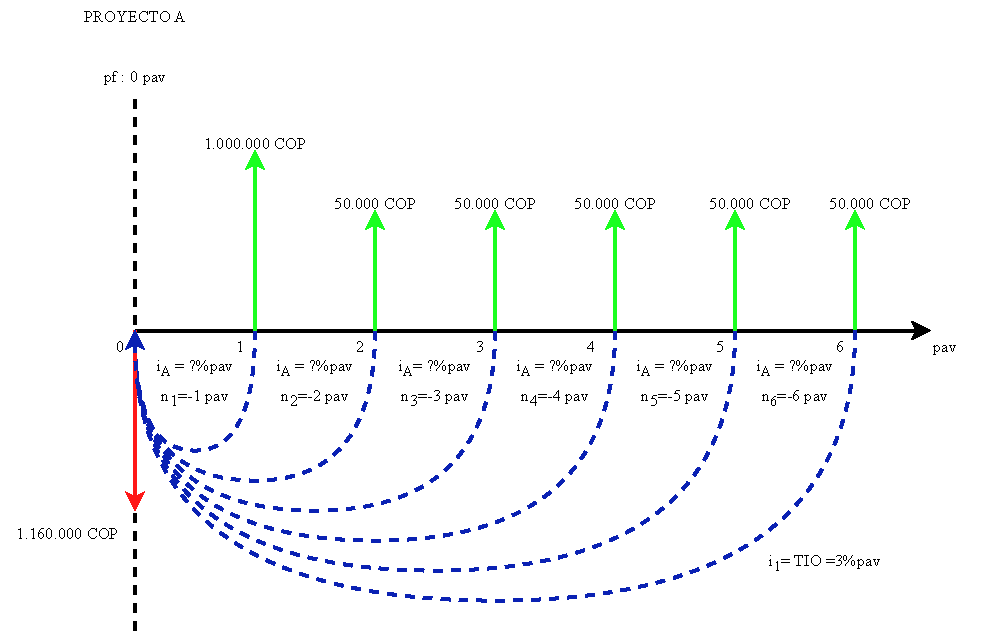
\includegraphics[scale=0.8]{ejemplos/2/Graf1Ej2Cap11.pdf} }                                                                                                \\
		\multicolumn{3}{|c|}{$ $}                                                                                                                                              \\
		\hline
		\multicolumn{3}{|c|}{$ $}                                                                                                                                              \\
		\multicolumn{3}{|c|}{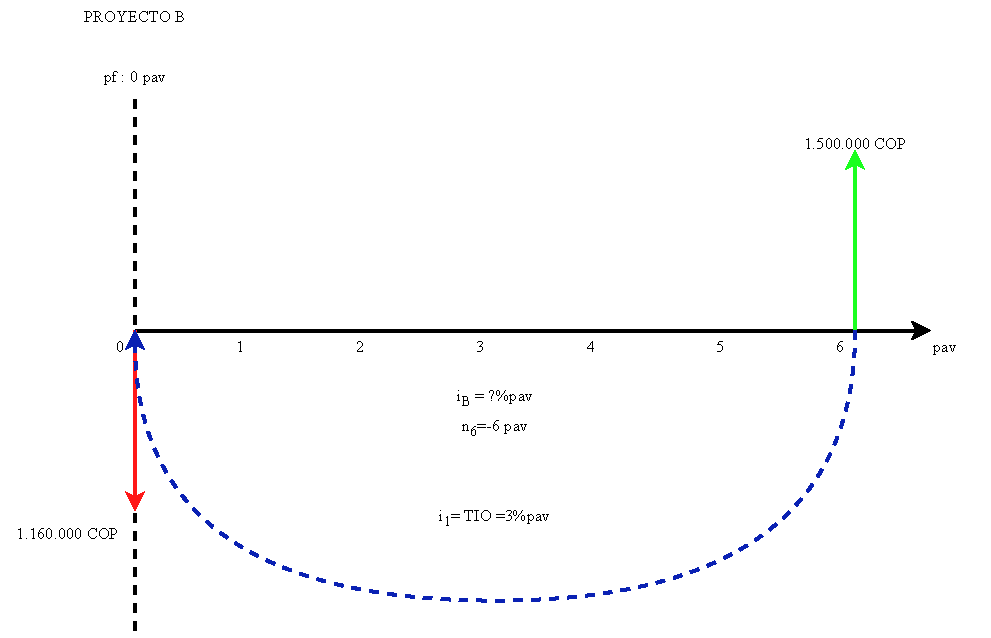
\includegraphics[scale=0.8]{ejemplos/2/Graf2Ej2Cap11.pdf} }

		\\\hline
		%%%%%%%%%%%%% FIN INSERCIÓN DE IMAGEN
		%%%%%FIN FLUJO DE CAJA



		%%%%% INICIO DECLARACIÓN FORMULAS
		%%%%%%%%%%% INICIO TITULO
		\rowcolor[HTML]{FFB183}
		\multicolumn{3}{|c|}{\cellcolor[HTML]{FFB183}\textbf{4. Declaración de fórmulas}}                                                                                      \\ \hline
		%%%%%%%%%%% FIN TITULO
		%%%%%%%%%%% INICIO MATEMÁTICAS
		\multicolumn{3}{|c|} {VPN =	$\sum F_{n}(1+i)^{-n}$   Valor presente neto.}                                                                                             \\ \hline

		%%%%%%%%%% FIN MATEMÁTICAS
		%%%%%% INICIO DESARROLLO MATEMÁTICO
		\rowcolor[HTML]{FFB183}
		%%%%%%%%%%INICIO TITULO
		\multicolumn{3}{|c|}{\cellcolor[HTML]{FFB183}\textbf{5. Desarrollo matemático}}                                                                                        \\ \hline
		%%%%%%%%%% FIN TITULO
		%%%%%%%%%% INICIO MATEMÁTICAS
		\multicolumn{3}{|c|}{$ \text{Análisis usando el VPN:} $}                                                                                                               \\
		\multicolumn{3}{|c|}{$ VPN(A) = -1\text{.}160\text{.}000\text{ COP} + 1\text{.}000\text{.}000\text{ COP}(1+0.03)^{-1} +$}                                              \\ \multicolumn{3}{|c|}{$50\text{.}000\text{ COP}(1+0.03)^{-2} + 50\text{.}000\text{ COP}(1+0.03)^{-3} + 50\text{.}000\text{ COP}(1+0.03)^{-4} $} \\
		\multicolumn{3}{|c|}{$ + 50\text{.}000\text{ COP}(1+0.03)^{-5} + 50\text{.}000\text{ COP}(1+0.03)^{-6} = 33\text{.}189.67\text{ COP.}$}                                \\
		\multicolumn{3}{|c|}{$ VPN(B) =- 1\text{.}160\text{.}000 \text{ COP} +  1\text{.}500\text{.}000(1+0.03)^{-6} = 96\text{.}226,38 \text{ COP.} $}                        \\
		\multicolumn{3}{|c|}{ $ \text{Análisis usando la TIR: } $}                                                                                                             \\
		\multicolumn{3}{|c|}{$ \text{Para calcular la TIR del proyecto A hacemos que VPN(A)=0 y dejamos la tasa como incógnita:}  $}                                           \\
		\multicolumn{3}{|c|}{$ VPN(A) = -1\text{.}160\text{.}000\text{ COP} + 1\text{.}000\text{.}000\text{ COP}(1+i_{A})^{-1} +$}                                             \\ \multicolumn{3}{|c|}{$50\text{.}000\text{ COP}(1+i_{A})^{-2} + 50\text{.}000\text{ COP}(1+i_{A})^{-3} + 50\text{.}000\text{ COP}(1+i_{A})^{-4} $} \\
		\multicolumn{3}{|c|}{$ + 50\text{.}000\text{ COP}(1+i_{A})^{-5} + 50\text{.}000\text{ COP}(1+i_{A})^{-6} = 0$}                                                         \\
		\multicolumn{3}{|c|}{$ \text{La solución manual requiere usar la interpolación, dando como resultado: } $}                                                             \\
		\multicolumn{3}{|c|}{$ i_{A} = TIR_{A} = 4.91\% pav$}                                                                                                                  \\
		\multicolumn{3}{|c|}{$ \text{Para calcular la TIR del proyecto B hacemos que VPN(B)=0 y dejamos la tasa como incógnita:}  $}                                           \\
		\multicolumn{3}{|c|}{$ VPN(B) =- 1\text{.}160\text{.}000 \text{ COP} +         1\text{.}500\text{.}000(1+i_{B})^{-6} = 0  $}                                           \\
		\multicolumn{3}{|c|}{$ \text{La solución manual requiere usar la interpolación, dando como resultado: } $}                                                             \\
		\multicolumn{3}{|c|}{$ i_{B} = TIR_{B} = 4.38\% pav$}                                                                                                                  \\

		\hline

		%%%%%%%%%% FIN MATEMÁTICAS
		%%%%%% FIN DESARROLLO MATEMÁTICO
		%%%%%% INICIO RESPUESTA
		\rowcolor[HTML]{FFB183}
		%%%%%%%%%%INICIO TITULO
		\multicolumn{3}{|c|}{\cellcolor[HTML]{FFB183}\textbf{6. Respuesta}}                                                                                                    \\ \hline
		%%%%%%%%%% FIN TITULO
		%%%%%%%%%% INICIO RESPUESTA MATEMÁTICA

		\multicolumn{3}{|c|}{ \text{El análisis usando el VPN indica que es mejor el proyecto B puesto que VPN(B)>VPN(A)} }                                                    \\
		\multicolumn{3}{|c|}{\text{El análisis usando la TIR indica que es mejor el proyecto A puesto que TIR(A)>TIR(B)}}                                                      \\
		\hline
		%%%%%%%%%% FIN MATEMÁTICAS
		%%%%%% FIN RESPUESTA
	\end{longtable}
	%Se crean dos lineas en blanco para que no quede el siguiente texto tan pegado
	%\newline \newline %USARLO SI CREES QUE ES NECESARIO
\end{center}
%%%%%%%%%%%%%%%%%%%%%%%%%%FIN EJERCICIO 2 %%%%%%%%%%%%%%%%%%%%%%%%%%%




\textbf{Disyuntiva VPN y TIR}\\
En el ejemplo anterior, según el índice VPN se debe optar por el proyecto B, pero según el índice TIR es mejor el proyecto A. Entonces ¿Cúal de los dos proyectos es mejor para invertir?\\
Para solucionar esta disyuntiva, hay que analizar lo que ocurre con los dineros que están invertidos en cada proyecto.\\

\begin{center}
	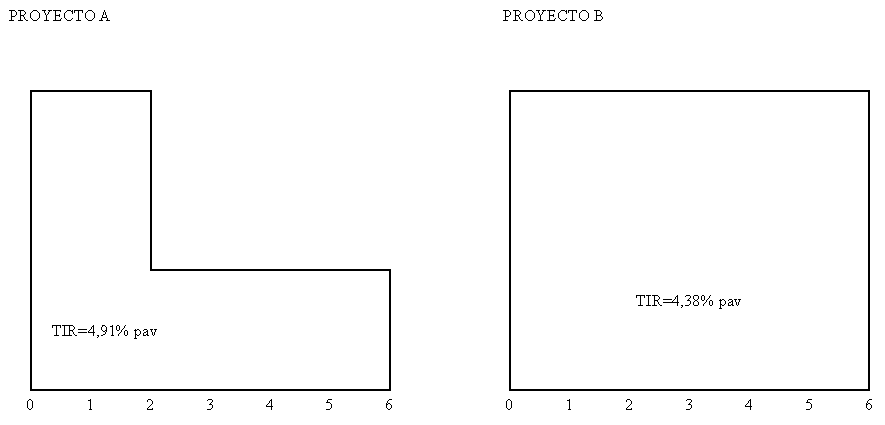
\includegraphics[scale=0.8]{explicacion/Graf4Cap11.pdf}
\end{center}
En el proyecto A la inversión de 1\text{.}160\text{.}000 COP solo dura un mes porque al cabo de un año está reintegrando 1\text{.}000\text{.}000 COP y en los 5 años restantes reintegra de a 50\text{.}000 COP anuales. En cambio en el proyecto B la inversión de 1\text{.}160\text{.}000 COP dura 6 años, y aunque estuvo colocado el dinero a una tasa menor el resultado final es que la ganancia en pesos de hoy es superior a la que genera el proyecto A.\\

El problema básicamente consiste en que la TIR solo mide la rentabilidad de los dineros que permanecen invertidos en el proyecto y no toma en cuenta los dineros que son liberados o los toma en cuenta suponiendo que los reinvierte a la misma tasa del proyecto lo cual es un error porque no necesariamente los dineros se reinvierten a la misma tasa del proyecto.\\

Para solucionar esta dificultad se debe tener en cuenta la reinversión y esta nueva TIR recibe el nombre de TIR Modificada que se representa por TIRM.\\

Se deja en claro que, la TIRM elimina la inconsistencia de ordenamiento entre la TIR y el VPN en la gran mayoría de los casos, sin embargo, quedan unos pocos casos en los cuales será necesario utilizar una variante de la TIRM que se denomina TIRM ponderada.\\

\textbf{Cálculo de la TIRM}\\

Se trasladan al punto inicial todos los egresos utilizando la tasa de financiación que puede ser la misma del mercado de colocación y se traslada a valor final todos los ingresos utilizando la tasa \textbf{TIO.}\\
Recordando que \textbf{TIO} es la tasa del mejor proyecto que se sacrifica a fin de realizar otra actividad.





\section{TIR + R}

Si los traslados de los ingresos a valor final y los traslados de los egresos a valor presente se hacen a una sola tasa, a la tasa del inversionista, esta TIR recibe el nombre de TIR+R que significa tasa interna de retorno con reinversión.

Al mirar la gráfica de flujo de caja del proyecto A se observa que solo hay un egreso y que además está ubicado en el punto inicial, entonces solo nos queda trasladar al punto 6 (punto final) todos los ingresos, y para ello utilizaremos una tasa del 3\% período anual vencido que es la tasa del inversionista.
\begin{center}
	$
		Ingresos = 1\text{.}000\text{.}000 COP(1+0.03)^{5}+ 50\text{.}000 COP(\frac{(1+0.03)^{5}-1}{0.03})=  1\text{.}424\text{.}730,87 COP
	$
\end{center}
%%\newpage
Nuestro flujo de caja queda modificado así:\\
\begin{center}
	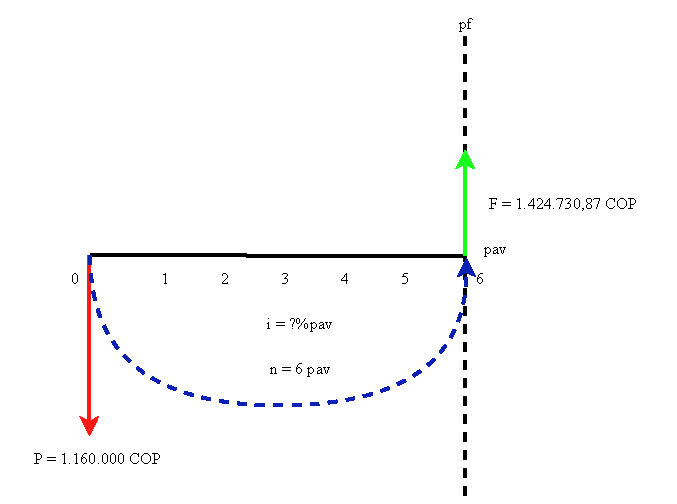
\includegraphics[scale=1.1]{explicacion/Graf3Cap11.pdf}
\end{center}
Utilizando la fórmula del interés compuesto podemos hallar la tasa del diagrama de flujo anterior así:
\begin{center}
	$\text{F} = P(1+i)^n \hspace{0.3cm} \textit{Valor futuro}$\\[0.5cm]
	$1\text{.}424\text{.}730,87 COP =  1\text{.}160\text{.}000 COP(1+i_{TIRM})^{6}$ \\[0.2cm]

\end{center}
De donde se obtiene que: TIRM(A) = 3,485\% período año vencido.\\

En el proyecto B TIRM es la misma TIR puesto que no ha habido oportunidad para hacer reinversiones, por lo tanto, TIRM(B) es igual a 4,38\% período año vencido y se concluye que si          TIRM(B) > TIRM(A) entonces el proyecto B es mejor que el proyecto A. Esta conclusión concuerda con la decisión que se toma usando el VPN como instrumento de análisis.\\

Hay ocasiones, aunque muy escasas, en que la TIRM aún no es suficiente para producir el mismo ordenamiento que el que produce el VPN, esto podría presentarse al comparar alternativas mutuamente excluyentes que tienen diferente costo, en tales circunstancias debemos hacer que las alternativas tengan el mismo costo y para ello le agregamos a la alternativa de menor costo una inversión adicional por un valor igual a la diferencia entre las dos alternativas. Esta alternativa adicional se evalúa a la tasa TIO.\\


\textbf{Ejemplo 3}\\

Supongamos que hay en estudio dos opciones de inversión: el proyecto A que requiere una inversión inicial de 200.000 COP y produce un ingreso de 31.160 COP durante 10 períodos y el proyecto B que tiene un costo de  100.000 COP y produce un ingreso durante 10 períodos de 16.280 COP. Se tiene una tasa de oportunidad del 5\% período mes vencido. Determinar cual es el mejor proyecto.
\\

\textbf{Solución.}\\
%La tabla ira centrada
\begin{center}
	\renewcommand{\arraystretch}{1.5}% Margenes de las celdas
	%Creación de la cuadricula de 3 columnas
	\begin{longtable}[H]{|c|c|c|}
		%Creamos una linea horizontal
		\hline
		%Definimos el color de la primera fila
		\rowcolor[HTML]{FFB183}
		%%%%% INICIO ASIGNACIÓN PERÍODO FOCAL %%%%%%%
		%%%%%%%%%% INICIO TITULO
		%Lo que se hace aquí es mezclar las 3 columnas en una sola
		\multicolumn{3}{|c|}{\cellcolor[HTML]{FFB183}\textbf{1. Asignación período focal}}                                                            \\ \hline
		%%%%%%%%%% FIN TITULO
		%%%%% INICIO DECLARACIÓN DE VARIABLES %%%%%%%
		\multicolumn{3}{|c|}{$pf : 0 pmv$}                                                                                                            \\ \hline

		%%%%%%%%%%% INICIO TITULO
		\rowcolor[HTML]{FFB183}
		\multicolumn{3}{|c|}{\cellcolor[HTML]{FFB183}\textbf{2. Declaración de variables}}                                                            \\ \hline
		%%%%%%%%%%% FIN TITULO
		%%%%%%%%%%% INICIO MATEMÁTICAS

		$\textbf{Proyecto A}$                                      & \multicolumn{2}{c|}{$ \textbf{Proyecto B} $}                                     \\
		$i = TIO = 5\% $ $ pmv  \hspace{0.3cm} $                   & \multicolumn{2}{c|}{$ i  = TIO  = 5\% pmv$}                                      \\
		$ n = 10 pmv $                                             & \multicolumn{2}{c|}{ $ n = 10 pmv $ }                                            \\
		$\text{Inversión inicial} = 200\text{.}000$ $COP $         & \multicolumn{2}{c|}{ $ \text{Inversión inicial} =  100\text{.}000$ $COP$}        \\
		$ \text{Ingreso por 10 periodos} =  31\text{.}160$ $ COP $ & \multicolumn{2}{c|}{ $ \text{Ingreso por 10 periodos} = 16\text{.}280$ $ COP $ }
		\\
		$  $                                                       & \multicolumn{2}{c|}{ $ $ }
		\\
		\hline
		%%%%%%%%%% FIN MATEMÁTICAS
		%%%%% INICIO FLUJO DE CAJA
		\rowcolor[HTML]{FFB183}
		\multicolumn{3}{|c|}{\cellcolor[HTML]{FFB183}\textbf{3. Diagrama de flujo de caja}}                                                           \\ \hline
		%Mezclamos 3 columnas y pondremos el dibujo
		%%%%%%%%%%%%% INSERCIÓN DE LA IMAGEN
		%Deberán descargar las imágenes respectivas del drive y pegarlas en la carpeta
		%n_capitulo/img/ejemplos/1/capitulo1ejemplo1.pdf  (el /1/ es el numero del ejemplo)
		\multicolumn{3}{|c|}{ 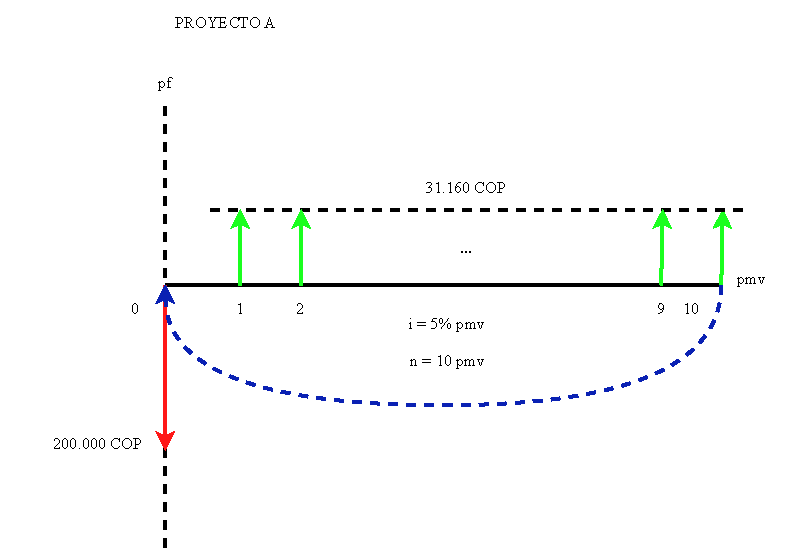
\includegraphics[scale=1]{ejemplos/3/Graf1Ej3Cap11.pdf} }
		\\
		\multicolumn{3}{|c|}{ 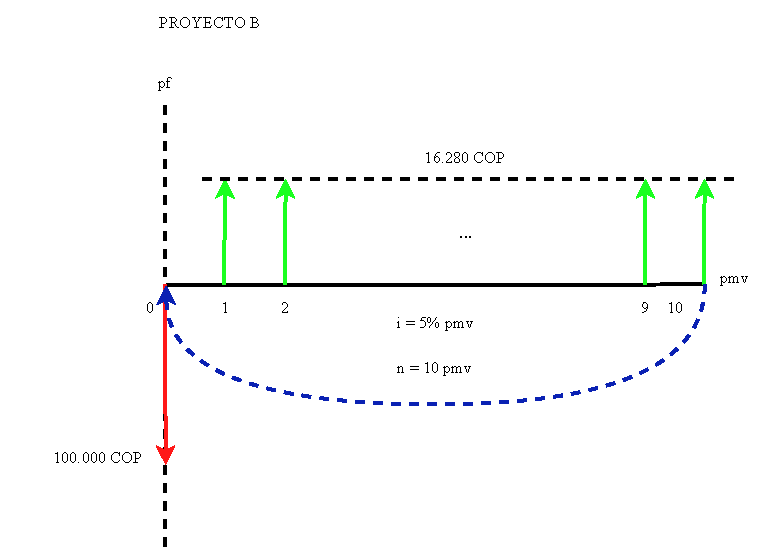
\includegraphics[scale=1]{ejemplos/3/Graf2Ej3Cap11.pdf} }
		\\\hline
		%%%%%%%%%%%%% FIN INSERCIÓN DE IMAGEN
		%%%%%FIN FLUJO DE CAJA



		%%%%% INICIO DECLARACIÓN FORMULAS
		%%%%%%%%%%% INICIO TITULO
		\rowcolor[HTML]{FFB183}
		\multicolumn{3}{|c|}{\cellcolor[HTML]{FFB183}\textbf{4. Declaración de fórmulas}}                                                             \\ \hline
		%%%%%%%%%%% FIN TITULO
		%%%%%%%%%%% INICIO MATEMÁTICAS
		\multicolumn{3}{|c|} {VPN =	$\sum F_{n}(1+i)^{-n}$   Valor presente neto.}                                                                    \\ \hline

		%%%%%%%%%% FIN MATEMÁTICAS
		%%%%%% INICIO DESARROLLO MATEMÁTICO
		\rowcolor[HTML]{FFB183}
		%%%%%%%%%%INICIO TITULO
		\multicolumn{3}{|c|}{\cellcolor[HTML]{FFB183}\textbf{5. Desarrollo matemático}}                                                               \\ \hline
		%%%%%%%%%% FIN TITULO
		%%%%%%%%%% INICIO MATEMÁTICAS
		\multicolumn{3}{|c|}{$ VPN(A)=- 200\text{.}000 COP + 31\text{.}160 COP(\frac{1-(1+0.05)^{-10}}{0.05})= $ $ 40\text{.}609,26 COP$}
		\\

		\multicolumn{3}{|c|}{$ VPN(B)=- 100\text{.}000 COP + 16\text{.}280 COP(\frac{1-(1+0.05)^{-10}}{0.05})=$ $ 25\text{.}709,84 COP$}
		\\\hline
		\multicolumn{3}{|c|}{$ \textbf{El VPN nos dice que es mejor el proyecto A}$}
		\\
		\multicolumn{3}{|c|}{$ \textbf{Evaluando el TIR}$}
		\\
		\multicolumn{3}{|c|}{$ TIR(A) = -200\text{.}000 COP + 31\text{.}160 COP(\frac{1-(1+i)^{-10}}{0.05})= $ $ 0 COP$}
		\\
		\multicolumn{3}{|c|}{$ \text{Calculando i por interpolación se tiene que TIR(A)=9\% pmv} $}
		\\
		\multicolumn{3}{|c|}{$ TIR(B)=- 100\text{.}000 COP + 16\text{.}280 COP(\frac{1-(1+i)^{-10}}{0.05}) = $ $ 0 COP$}
		\\
		\multicolumn{3}{|c|}{$ \text{Calculando i por interpolación se tiene que TIR(B)=10,01\% pmv} $}
		\\
		\multicolumn{3}{|c|}{$ \text{La TIR nos dice que es mejor el proyecto B, lo cual contradice al VPN.} $}
		\\
		\multicolumn{3}{|c|}{$ \text{Intentamos aclarar esta contradicción usando la TIRM.} $}
		\\
		\multicolumn{3}{|c|}{$ \textbf{Evaluando la TIRM } $}
		\\
		\multicolumn{3}{|c|}{$ \text{TIRM(A):  Trasladamos a valor final la serie de 10 ingresos de 31.160 COP y tenemos:} $}
		\\
		\multicolumn{3}{|c|}{$ 31\text{.}160 COP(\frac{(1+0.05)^{10}-1}{0.05}) = $ $ 391\text{.}927,13 COP  \textbf{ Ecuación de equivalencia }$}
		\\
		\multicolumn{3}{|c|}{ 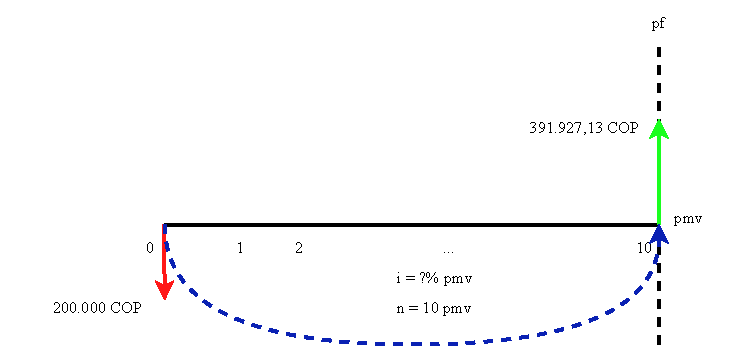
\includegraphics[scale=1]{ejemplos/3/Graf3Ej3Cap11.pdf} }
		\\
		\multicolumn{3}{|c|}{$391\text{.}927,13 COP =  200\text{.}000 COP(1+i)^{10}$}
		\\
		\multicolumn{3}{|c|}{$ i=TIRM(A)=6.96\% pmv$}
		\\
		\multicolumn{3}{|c|}{$ \text{TIRM(B):  Trasladamos a valor final la serie de 10 ingresos de 16.280 COP y tenemos:} $}
		\\
		\multicolumn{3}{|c|}{$ 16\text{.}280 COP(\frac{(1+0.05)^{10}-1}{0.05}) = 204\text{.}768,1 COP  \textbf{    Ecuación de equivalencia }$}
		\\
		\multicolumn{3}{|c|}{ 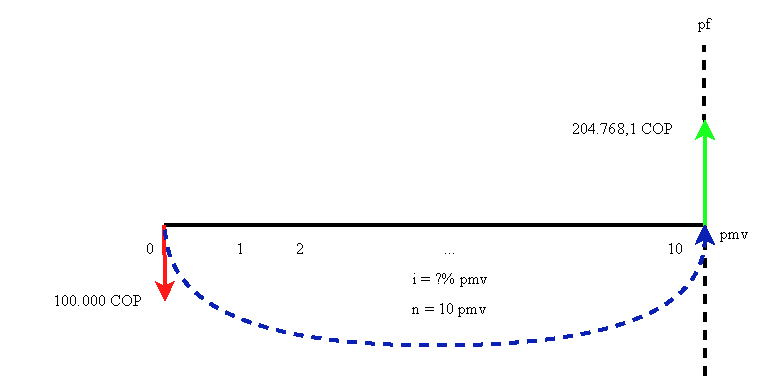
\includegraphics[scale=1]{ejemplos/3/Graf4Ej3Cap11.pdf} }
		\\
		\multicolumn{3}{|c|}{$ 204\text{.}768,1 COP = 100\text{.}000 COP(1+i)^{10}$}
		\\
		\multicolumn{3}{|c|}{$i=TIRM(B)=7.43\% pmv$}
		\\
		\multicolumn{3}{|c|}{$\text{Se concluye que TIRM(B) es mejor que TIRM(A)}$}
		\\
		\multicolumn{3}{|c|}{$\text{Como el proyecto A es más costoso que el proyecto B }$}
		\\
		\multicolumn{3}{|c|}{$\text{debemos adicionar al proyecto B  el proyecto adicional con inversión inicial de 100.000 COP y }$}
		\\
		\multicolumn{3}{|c|}{$\text{lo evaluaremos a la tasa del 5\% pmv.}$}
		\\
		\multicolumn{3}{|c|}{$ 100\text{.}000 COP(1+0.05)^{10} = 162\text{.}889,46 COP$}
		\\
		\multicolumn{3}{|c|}{ 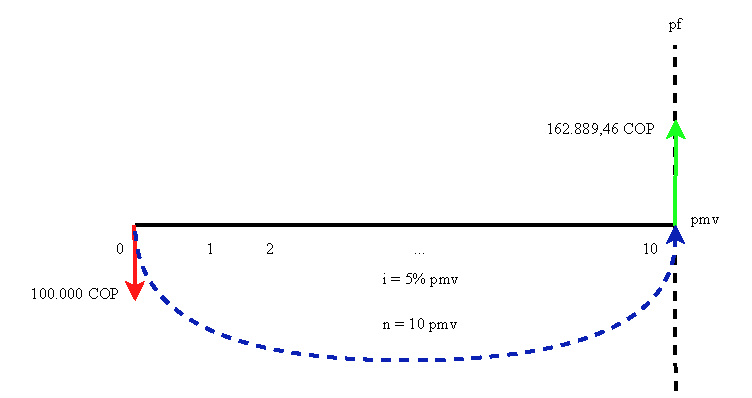
\includegraphics[scale=1]{ejemplos/3/Graf5Ej3Cap11.pdf} }
		\\
		\multicolumn{3}{|c|}{$\text{Entonces el nuevo proyecto B quedará formado por el proyecto B incial   }$}
		\\
		\multicolumn{3}{|c|}{$\text{más el proyecto adicional con el siguiente flujo de caja:  }$}
		\\
		\multicolumn{3}{|c|}{$\textbf{Ingresos en el periodo 10: } 204\text{.}768,1 COP + 162\text{.}889,46 COP = 367\text{.}657,56 COP$}
		\\
		\multicolumn{3}{|c|}{$\textbf{Costo inicial: } 100\text{.}000 COP + 100\text{.}000 COP = 200\text{.}000 COP$}
		\\
		\multicolumn{3}{|c|}{ 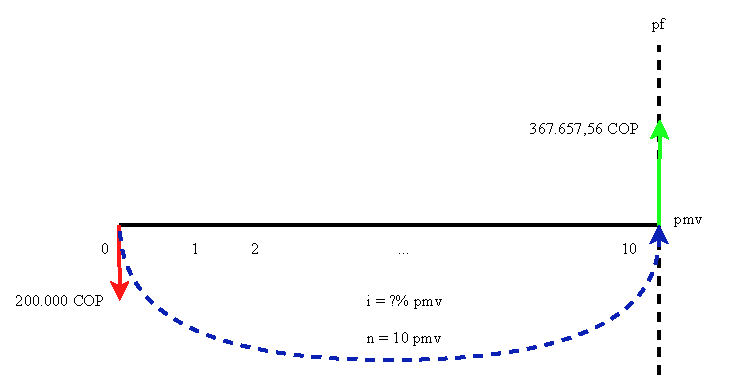
\includegraphics[scale=1]{ejemplos/3/Graf6Ej3Cap11.pdf} }
		\\
		\multicolumn{3}{|c|}{$\text{ Ahora calculamos la TIR de este nuevo proyecto así: } $}
		\\
		\multicolumn{3}{|c|}{$367\text{.}657,56 COP = 200\text{.}000 COP(1+i)^{10}$}
		\\
		\multicolumn{3}{|c|}{ \text{Al despejar se tiene que i = TIR(B) = 6,28\% pmv, el cual es inferior a la TIR(A)}}
		\\
		\hline

		%%%%%%%%%% FIN MATEMÁTICAS
		%%%%%% FIN DESARROLLO MATEMÁTICO
		%%%%%% INICIO RESPUESTA
		\rowcolor[HTML]{FFB183}
		%%%%%%%%%%INICIO TITULO
		\multicolumn{3}{|c|}{\cellcolor[HTML]{FFB183}\textbf{6. Respuesta}}                                                                           \\ \hline
		%%%%%%%%%% FIN TITULO
		%%%%%%%%%% INICIO RESPUESTA MATEMÁTICA

		\multicolumn{3}{|c|}{ \text{Es mejor invertir en el proyecto A que en el proyecto B, ya que la TIR y }}
		\\
		\multicolumn{3}{|c|}{ \text{VPN del proyecto A son mayores que la TIR y VPN del proyecto B respectivamente.}}
		\\
		\hline


		%%%%%%%%%% FIN MATEMÁTICAS
		%%%%%% FIN RESPUESTA
	\end{longtable}
	%Se crean dos lineas en blanco para que no quede el siguiente texto tan pegado
	%\newline \newline %USARLO SI CREES QUE ES NECESARIO
\end{center}
%%%%%%%%%%%%%%%%%%%%%%%%%%FIN EJERCICIO 1 %%%%%%%%%%%%%%%%%%%%%%%%%%%

El lector observará que hemos buscado por diferentes caminos que los dos ordenamientos coincidan. \\
Cuando los instrumentos de análisis VPN y TIR producen diferentes resultados es porque se ha cometido un error en la forma de aplicar la TIR. El verdadero ordenamiento es el que produce el VPN, por esta razón debe calcularse la TIR por diferentes métodos hasta que esté de acuerdo con el ordenamiento del VPN (el valor de la TIRM siempre se encuentra entre la TIR y la tasa de reinversión).\\

\subsubsection{TIR múltiple}

En un proyecto, el flujo de caja puede darse de dos maneras: primero, pueden haber egresos (uno o varios) y después aparecen los ingresos (uno o varios). Este tipo de proyectos recibe el nombre de proyectos convencionales y solo tienen una tasa, pero puede suceder que en un proyecto los egresos y los ingresos aparezcan en forma entreverada, en este caso puede suceder que existan varias tasas y el proyecto recibe el nombre de no convencional.

%desde aca empiezo yo ------------------- $
\section{Regla de los signos de Descartes}


Un polinomio ordenado es aquel en que los exponentes están en orden ascendente o en orden descendente, por ejemplo: \\

\begin{center}
	$3x^{6}+12x^{4}-25x^{3}+16x+35=0$
\end{center}

Podemos asumir que los términos en $x^{5}$  y en $x^{2}$ tienen coeficiente igual a cero por eso no figuran. \\

Según Descartes, un polinomio ordenado no tiene más raíces positivas que el número de veces en que los coeficientes cambian de signo, esto significa que la ecuación anterior a lo sumo tiene 2 raíces porque los dos primeros términos son positivos, el tercer término es negativo, esto implica un cambio de signo, el cuarto término vuelve a ser positivo lo cual implica otro cambio de signo y el quinto término sigue siendo positivo, en consecuencia en total hay dos cambios de signo y esto significa que a lo sumo habrá 2 raíces. (Los sitios donde los coeficientes cambian de signo se señalan con flechas)\\

\textbf{Observación:} Al decir que a lo sumo hay 2 raíces positivas, significa que puede haber una sola raíz o que haya 2 raíces positivas, pero en ningún caso puede haber más de 2 raíces positivas o que haya ninguna raíz positiva.\\
%Evitar negar dos veces en la observación anterior.

Otro ejemplo:
\begin{center}
	$
		26(1+i)^{-7}+2(1+i)^{-3}-\underbrace{14(1+i)^{-2}}_{}+\underbrace{16(1+i)^{-1}}_{}-\underbrace{40}_{}=0
	$
\end{center}

La ecuación anterior a lo sumo tiene 3 raíces positivas porque hay tres cambios de signo en los coeficientes, los cuales hemos señalado con los corchetes. \\

Cuando se trabaja manualmente la mejor forma de encontrar las raíces es construir la gráfica de la ecuación y las raíces son aquellos puntos de corte de la curva sobre el eje X. Cuando trabajamos manualmente no nos interesa construir la parte negativa del eje X porque una raíz negativa significa que un proyecto tiene una tasa negativa, es decir, que si se realiza el proyecto va a dar una pérdida y no es lógico que una persona invierta un dinero con la intención de perder. \\

Como comentario adicional, una ecuación que tenga una curva de la siguiente forma: \\
\textbf{Figura 3} \\
\textit{Curva con raíz imaginaria y raíz real negativa}
\begin{center}
	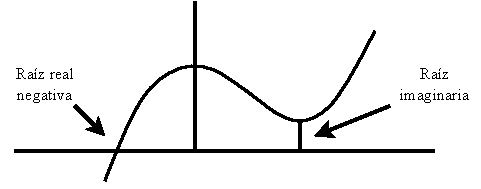
\includegraphics[scale=1]{explicacion/Graf5Cap11.pdf}
\end{center}

Matemáticamente, tiene una raíz negativa y una raíz imaginaria. El campo de las finanzas no tiene raíces porque ya dijimos que descartábamos las raíces negativas y además debemos descartar las raíces imaginarias porque en finanzas solo se trabaja con los números reales.\\

Ahora estudiemos la forma de encontrar el valor de las raíces, para ello tomemos el siguiente caso: \\\\

\textbf{Ejemplo 4}\\

Un proyecto requiere una inversión inicial de 40.000 COP, en el período 1 los ingresos son iguales a los egresos, en el período 2 hay un ingreso neto de 100.000 COP, en los períodos 3 y 4 los ingresos y los egresos vuelven a dar un flujo de caja neto de 0, finalmente en el período 5 hay un egreso de 60.000 COP. Calcular la TIRM del proyecto.
\\

\textbf{Solución.}
%La tabla ira centrada
\begin{center}
	\renewcommand{\arraystretch}{1.5}% Margenes de las celdas
	%Creación de la cuadricula de 3 columnas
	\begin{longtable}[H]{|c|c|c|}
		%Creamos una linea horizontal
		\hline
		%Definimos el color de la primera fila
		\rowcolor[HTML]{FFB183}
		%%%%% INICIO ASIGNACIÓN PERÍODO FOCAL %%%%%%%
		%%%%%%%%%% INICIO TITULO
		%Lo que se hace aquí es mezclar las 3 columnas en una sola
		\multicolumn{3}{|c|}{\cellcolor[HTML]{FFB183}\textbf{1. Asignación período focal}}                                                                                                                                         \\ \hline
		%%%%%%%%%% FIN TITULO
		%%%%% INICIO DECLARACIÓN DE VARIABLES %%%%%%%
		\multicolumn{3}{|c|}{$pf : 0 pmv$}                                                                                                                                                                                         \\ \hline

		%%%%%%%%%%% INICIO TITULO
		\rowcolor[HTML]{FFB183}
		\multicolumn{3}{|c|}{\cellcolor[HTML]{FFB183}\textbf{2. Declaración de variables}}                                                                                                                                         \\ \hline
		\hline
		
		\rowcolor[HTML]{FFB183}
		\multicolumn{1}{|c|}{\cellcolor[HTML]{FFB183}\textbf{Valores monetarios}} & \multicolumn{1}{c|}{\cellcolor[HTML]{FFB183}\textbf{Valores no monetarios}} & \multicolumn{1}{c|}{\cellcolor[HTML]{FFB183}\textbf{Incógnitas}} \\ \hline
		%%%%%%%%%%% FIN TITULO
%%%%%%%%%%% INICIO MATEMÁTICAS
\text{Inversión inicial} = \text{ 40.000 COP}                            & $n = 5 pmv$                                                                 & $TIRM= ?\% pmv$                                                  \\
\text{Periodo 2 ingreso} = \text{ 100.000 COP}                           &                                                                             &                                                                  \\
\text{Periodo 5 ingreso} = \text{ 60.000 COP}                            &                                                                             &                                                                  \\
\hline
%%%%%%%%%% FIN MATEMÁTICAS

		%%%%% INICIO FLUJO DE CAJA
		\rowcolor[HTML]{FFB183}
		\multicolumn{3}{|c|}{\cellcolor[HTML]{FFB183}\textbf{3. Diagrama de flujo de caja}}                                                                                                                                        \\ \hline
		%Mezclamos 3 columnas y pondremos el dibujo
		%%%%%%%%%%%%% INSERCIÓN DE LA IMAGEN
		%Deberán descargar las imágenes respectivas del drive y pegarlas en la carpeta
		%n_capitulo/img/ejemplos/1/capitulo1ejemplo1.pdf  (el /1/ es el numero del ejemplo)
		\multicolumn{3}{|c|}{ 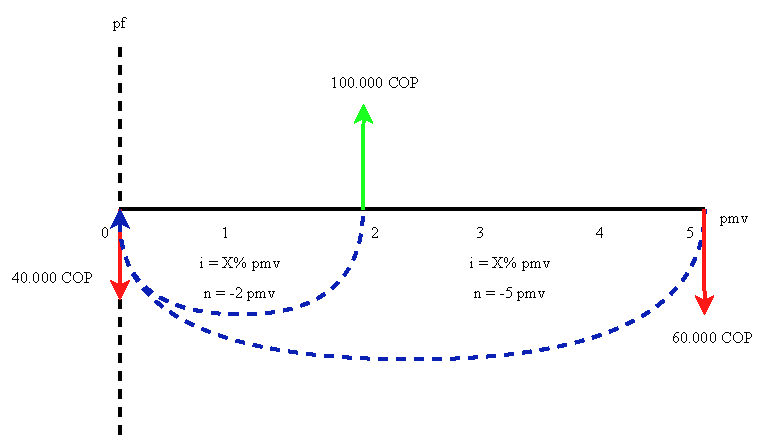
\includegraphics[scale=1]{ejemplos/4/Graf1Ej4Cap11.pdf} }
		\\\hline
		%%%%%%%%%%%%% FIN INSERCIÓN DE IMAGEN
		%%%%%FIN FLUJO DE CAJA



		%%%%% INICIO DECLARACIÓN FORMULAS
		%%%%%%%%%%% INICIO TITULO
		\rowcolor[HTML]{FFB183}
		\multicolumn{3}{|c|}{\cellcolor[HTML]{FFB183}\textbf{4. Declaración de fórmulas}}                                                                                                                                          \\ \hline
		%%%%%%%%%%% FIN TITULO
		%%%%%%%%%%% INICIO MATEMÁTICAS
		\multicolumn{3}{|c|} {VPN =	$\sum F_{n}(1+i)^{-n}$   Valor presente neto.}                                                                                                                                                 \\
		\multicolumn{3}{|c|} { $ i= j/m $ Tasa anualizada. }                                                                                                                                                                        \\

		\hline

		%%%%%%%%%% FIN MATEMÁTICAS
		%%%%%% INICIO DESARROLLO MATEMÁTICO
		\rowcolor[HTML]{FFB183}
		%%%%%%%%%%INICIO TITULO
		\multicolumn{3}{|c|}{\cellcolor[HTML]{FFB183}\textbf{5. Desarrollo matemático}}                                                                                                                                            \\ \hline
		%%%%%%%%%% FIN TITULO
		%%%%%%%%%% INICIO MATEMÁTICAS
		\multicolumn{3}{|c|}{-$40\text{.}000 COP   +  100\text{.}000 COP(1+i)^{-2}$ - $  60\text{.}000 COP(1+i)^{-5} = 0 COP$}
		\\

		\multicolumn{3}{|c|}{$ \text{Construimos una tabla de valores X,Y para ver el comportamiento de la gráfica y así determinar}$}
		\\
		\multicolumn{3}{|c|}{$ \text{las tasas:} $}
		\\

		\hline
		$ $                                                                       & \multicolumn{2}{c|}{ }                                                                                                                         \\

		{\fontsize{9}{10}\selectfont
		\setlength{\arrayrulewidth}{0.2mm} % Aumentar el grosor de las líneas
		\renewcommand{\arraystretch}{1.5} % Aumentar la altura de las filas
		\begin{tabular}{|>{\centering\arraybackslash}p{3cm}|>{\centering\arraybackslash}p{2cm}|}
			\hline
			\rowcolor{white!50}
			\textbf{X}     & \textbf{Y}  \\ \hline
			\text{0\%pmv}  & \text{0}    \\ \hline
			\text{10\%pmv} & \text{5,39} \\ \hline
			\text{20\%pmv} & \text{5,33} \\ \hline
			\text{30\%pmv} & \text{3,01} \\ \hline
			\text{40\%pmv} & \text{-135} \\ \hline
		\end{tabular}
		}
		                                                                          & \multicolumn{2}{c|}{{\fontsize{9}{10}\selectfont
					\setlength{\arrayrulewidth}{0.2mm} % Aumentar el grosor de las líneas
					\renewcommand{\arraystretch}{1.5} % Aumentar la altura de las filas
					\begin{tabular}{|>{\centering\arraybackslash}p{2cm}|>{\centering\arraybackslash}p{2cm}|}
						\hline
						\rowcolor{white!50}
						\textbf{X}     & \textbf{Y}      \\ \hline
						\text{39\%pmv} & \text{193,976}  \\ \hline
						\text{40\%pmv} & \text{-135,658} \\ \hline
					\end{tabular}
		}}                                                                                                                                                                                                                         \\
		$ $                                                                       & \multicolumn{2}{c|}{ }                                                                                                                         \\
		\hline
		\multicolumn{3}{|c|}{ }                                                                                                                                                                                                    \\

		\multicolumn{3}{|c|}{ \scalebox{1}{$\displaystyle\frac{39\%-40\%}{39\%-X} = \frac{193\text{,}976-(-135\text{,}658)}{193\text{,}975-0} $ }}
		\\
		\multicolumn{3}{|c|}{\text{Al despejar se obtiene el valor de X que es igual a 39,588 \% pmv}}                                                                                                                             \\
		\multicolumn{3}{|c|}{\text{Los resultados indican que existen dos tasas, pero no se sabe cuál escoger.}}
		\\
		\multicolumn{3}{|c|}{$ \text{Suponiendo una tasa del 30\% pmv para la reinversión, los ingresos serán:} $}
		\\
		\multicolumn{3}{|c|}{$ 100\text{.}000 COP(1 + 0.3)^{3} = $ $ 219\text{.}700 COP $}
		\\
		\multicolumn{3}{|c|}{$ 40\text{.}000 COP + 60\text{.}000 COP(1+0.25)^{-5} = $ $  59\text{.}660.80 COP $}                                                                                                                   \\ \hline
		\hline
		\multicolumn{3}{|c|}{$ \text{El nuevo diagrama de flujo de caja es:} $}
		\\
		\multicolumn{3}{|c|}{ 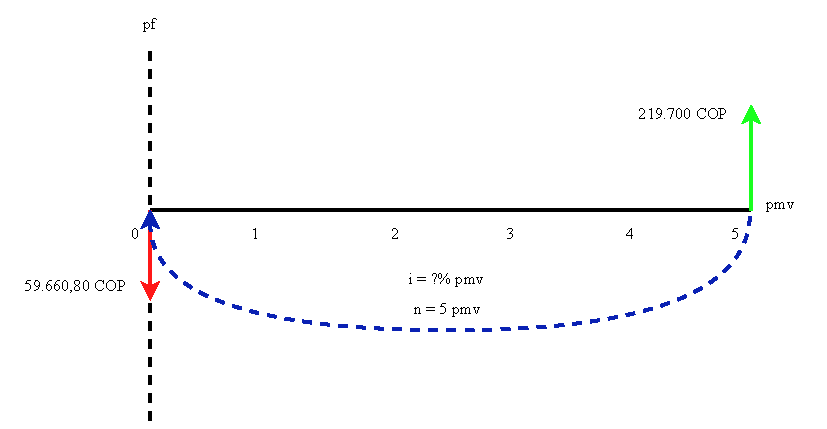
\includegraphics[scale=1]{ejemplos/4/Graf2Ej4Cap11.pdf} }
		\\
		\multicolumn{3}{|c|}{$ \text{Ahora se procede a calcular la TIRM:} $}
		\\
		\multicolumn{3}{|c|}{$219\text{.}700 COP = 59\text{.}660,80 COP(1+i)^{5} $}
		\\
		\multicolumn{3}{|c|}{$ TIRM = i = 29.786\% pmv $}
		\\
		\hline

		%%%%%%%%%% FIN MATEMÁTICAS
		%%%%%% FIN DESARROLLO MATEMÁTICO
		%%%%%% INICIO RESPUESTA
		\rowcolor[HTML]{FFB183}
		%%%%%%%%%%INICIO TITULO
		\multicolumn{3}{|c|}{\cellcolor[HTML]{FFB183}\textbf{6. Respuesta}}                                                                                                                                                        \\ \hline
		%%%%%%%%%% FIN TITULO
		%%%%%%%%%% INICIO RESPUESTA MATEMÁTICA

		\multicolumn{3}{|c|}{ \text{La TIRM del proyecto es igual a 29,786\% pmv}}
		\\

		\hline


		%%%%%%%%%% FIN MATEMÁTICAS
		%%%%%% FIN RESPUESTA
	\end{longtable}
	%Se crean dos lineas en blanco para que no quede el siguiente texto tan pegado
	%\newline \newline %USARLO SI CREES QUE ES NECESARIO
\end{center}
%%%%%%%%%%%%%%%%%%%%%%%%%%FIN EJERCICIO 1 %%%%%%%%%%%%%%%%%%%%%%%%%%%




\section{Tasa interna de retorno incremental TIRI}

Para calcular la TIR, es indispensable que existan tanto ingresos como egresos. Sin embargo, al seleccionar entre varias alternativas utilizando la TIR, puede darse el caso de proyectos mutuamente excluyentes en los cuales solo se conocen los egresos, pero no los ingresos o, en caso de conocerse, son mínimos en comparación con los egresos. En estas condiciones, no es posible conocer la rentabilidad de ninguno de los proyectos. Sin embargo, sí es posible obtener una rentabilidad de la diferencia entre las inversiones. Esta tasa se compara con la tasa mínima que el inversionista desea obtener, la cual representamos como TMAR, y nos ayuda a tomar una decisión.\\

\textbf{Ejemplo 5}\\

Dadas las alternativas A, B y C determinar la mejor alternativa usando el método de la TIRI
suponiendo que la TMAR= 25\% pmv, compruebe el resultado usando el VPN. Las inversiones iniciales y el costo anual de operación (CAO) son: \\

\begin{center}
	\begin{tabular}{|p{3.325cm}|p{3.325cm}| p{3.325cm}| p{3.325cm}|}
		\hline
		\begin{tabular}[c]{@{}c@{}}\textbf{Proyecto}\end{tabular} & \begin{tabular}[c]{@{}c@{}}\textbf{A} \end{tabular} & \begin{tabular}[c]{@{}c@{}}\textbf{B} \end{tabular} & \begin{tabular}[c]{@{}c@{}}\textbf{C} \end{tabular} \\ \hline

		Costo                                                     & 100.000  COP                                        & 120.000  COP                                        & 110.000  COP                                        \\ \hline

		CAO año 1                                                 & 10.000  COP                                         & 2.000    COP                                        & 5.500   COP                                         \\ \hline

		CAO año 2                                                 & 12.000  COP                                         & 3.000    COP                                        & 6.000    COP                                        \\ \hline

		CAO año 3                                                 & 14.000  COP                                         & 4.000    COP                                        & 7.000    COP                                        \\ \hline

		CAO año 4                                                 & 16.000   COP                                        & 5.000    COP                                        & 8.500    COP                                        \\ \hline
	\end{tabular}
\end{center}

\textbf{Solución:}\\
%La tabla ira centrada
\begin{center}
	\renewcommand{\arraystretch}{1.5}% Margenes de las celdas
	%Creación de la cuadricula de 3 columnas
	\begin{longtable}[H]{|c|c|c|}
		%Creamos una linea horizontal
		\hline
		%Definimos el color de la primera fila
		\rowcolor[HTML]{FFB183}
		%%%%% INICIO ASIGNACIÓN PERÍODO FOCAL %%%%%%%
		%%%%%%%%%% INICIO TITULO
		%Lo que se hace aquí es mezclar las 3 columnas en una sola
		\multicolumn{3}{|c|}{\cellcolor[HTML]{FFB183}\textbf{1. Asignación período focal}}                                  \\ \hline
		%%%%%%%%%% FIN TITULO
		%%%%% INICIO DECLARACIÓN DE VARIABLES %%%%%%%
		\multicolumn{3}{|c|}{$pf : 0 pmv$}                                                                                  \\ \hline

		%%%%%%%%%%% INICIO TITULO
		\rowcolor[HTML]{FFB183}
		\multicolumn{3}{|c|}{\cellcolor[HTML]{FFB183}\textbf{2. Declaración de variables}}                                  \\ \hline
		\multicolumn{1}{|c|}{\cellcolor[HTML]{FFB183}\textbf{Valores monetarios}} & \multicolumn{1}{c|}{\cellcolor[HTML]{FFB183}\textbf{Valores no monetarios}} & \multicolumn{1}{c|}{\cellcolor[HTML]{FFB183}\textbf{Incógnitas}} \\ \hline
		%%%%%%%%%%% FIN TITULO
		%%%%%%%%%%% INICIO MATEMÁTICAS

		$ \text{Inversión inicial} =   $ $ 20\text{.}000\text{ } COP $ & $ n = 5 pmv $ & $\text{i} = $ $?\text{ } COP$\\
		$ \text{Periodo 1 ingreso} = $ $8\text{.}000\text{ } COP $     & & $ VPN(A)=  ? \text{  } COP $\\
		$ \text{Periodo 2 ingreso} =  $ $ 9\text{.}000\text{ } COP $   & & $ VPN(B)= ?\text{  } COP   $\\
		$ \text{Periodo 3 ingreso} =   $ $ 10\text{.}000\text{ } COP $ & & $ VPN(C)=   ?\text{  } COP $\\
		$ \text{Periodo 4 ingreso} =   $ $ 11\text{.}000\text{ } COP $ & & \\
		\hline
		%%%%%%%%%% FIN MATEMÁTICAS
		%%%%% INICIO FLUJO DE CAJA
		\rowcolor[HTML]{FFB183}
		\multicolumn{3}{|c|}{\cellcolor[HTML]{FFB183}\textbf{3. Diagrama de flujo de caja}}                                 \\ \hline
		%Mezclamos 3 columnas y pondremos el dibujo
		%%%%%%%%%%%%% INSERCIÓN DE LA IMAGEN
		%Deberán descargar las imágenes respectivas del drive y pegarlas en la carpeta
		%n_capitulo/img/ejemplos/1/capitulo1ejemplo1.pdf  (el /1/ es el numero del ejemplo)
		\multicolumn{3}{|c|}{ 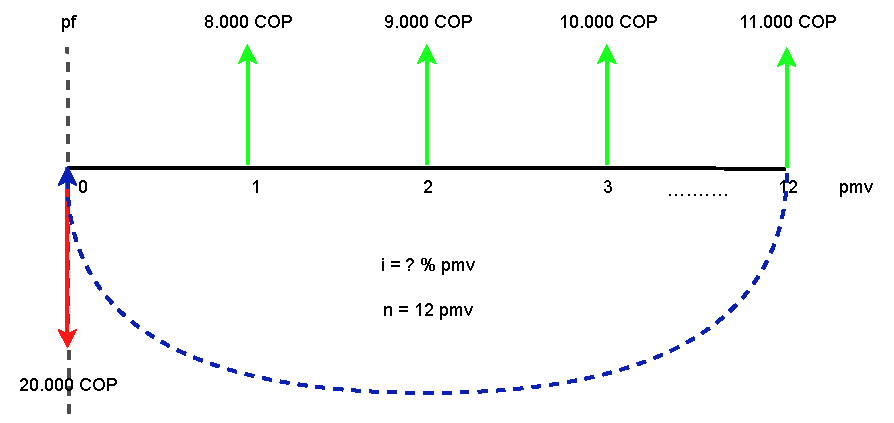
\includegraphics[scale=0.8, trim=0cm -0.5cm 0.0cm -0.5cm]{ejemplos/5/Graf1Ej5Cap11.pdf} }                                              \\\hline
		%%%%%%%%%%%%% FIN INSERCIÓN DE IMAGEN
		%%%%%FIN FLUJO DE CAJA



		%%%%% INICIO DECLARACIÓN FORMULAS
		%%%%%%%%%%% INICIO TITULO
		\rowcolor[HTML]{FFB183}
		\multicolumn{3}{|c|}{\cellcolor[HTML]{FFB183}\textbf{4. Declaración de fórmulas}}                                   \\ \hline
		%%%%%%%%%%% FIN TITULO
		%%%%%%%%%%% INICIO MATEMÁTICAS
		\multicolumn{3}{|c|} {VPN =	$\sum F_{n}(1+i)^{-n}$   Valor presente neto.}                                          \\
		\multicolumn{3}{|c|} {i  $=j/m$ tasa periodica. }                                                                    \\
		\hline

		%%%%%%%%%% FIN MATEMÁTICAS
		%%%%%% INICIO DESARROLLO MATEMÁTICO
		\rowcolor[HTML]{FFB183}
		%%%%%%%%%%INICIO TITULO
		\multicolumn{3}{|c|}{\cellcolor[HTML]{FFB183}\textbf{5. Desarrollo matemático}}                                     \\ \hline

		%%\multicolumn{3}{|c|}{ \includegraphics[scale=0.7]{5/Graf2Ej5Cap11.pdf} }
		\multicolumn{3}{|c|}{}                                                                                              \\
		\multicolumn{3}{|c|}{
			{\fontsize{9}{10}\selectfont
					\begin{tabular}{|>{\centering\arraybackslash}p{3cm}|>{\centering\arraybackslash}p{3cm}|>{\centering\arraybackslash}p{3cm}|>{\centering\arraybackslash}p{3cm}|}
						\hline
						\rowcolor{white!50}
						\textbf{Periodo} & \textbf{A}                 & \textbf{B}                 & \textbf{B - A}            \\ \hline
						\text{0}         & \text{-100\text{.}000 COP} & \text{-120\text{.}000 COP} & \text{-20\text{.}000 COP} \\ \hline
						\text{1}         & \text{-10\text{.}000 COP}  & \text{-2\text{.}000 COP}   & \text{+8\text{.}000 COP}  \\ \hline
						\text{2}         & \text{-12\text{.}000 COP}  & \text{-3\text{.}000 COP}   & \text{+9\text{.}000 COP}  \\ \hline
						\text{3}         & \text{-14\text{.}000 COP}  & \text{-4\text{.}000 COP}   & \text{+10\text{.}000 COP} \\ \hline
						\text{4}         & \text{-16\text{.}000 COP}  & \text{-5\text{.}000 COP}   & \text{+11\text{.}000 COP} \\ \hline
					\end{tabular}
				}
		}                                                                                                                   \\
		\multicolumn{3}{|c|}{ }                                                                                             \\
		%%%%%%%%%% FIN TITULO
		%%%%%%%%%% INICIO MATEMÁTICAS
		\multicolumn{3}{|c|}{$ VPN(B-A): -   20\text{.}000\text{ } COP +   8\text{.}000(1+i)^{-1}\text{ } COP +    9\text{.}000(1 +i)^{-2}\text{ } COP +$}
		\\
		\multicolumn{3}{|c|}{$  10\text{.}000(1 +i)^{-3}\text{ } + COP 11\text{.}000(1+0)^{-4}\text{ } COP =   $ 0 $\text{ }  COP$ }
		\\
		\multicolumn{3}{|c|}{$ \text{Como la TIRI es mayor a la TMAR se concluye que el exceso } $}
		\\
		\multicolumn{3}{|c|}{$ \text{de inversión (20.000  COP ) genera un interés del} $}
		\\
		\multicolumn{3}{|c|}{$ \text{29,67\% pmv superior a la TMAR que es del 25\% pmv}$}
		\\
		\multicolumn{3}{|c|}{$ \textbf{Observe que tenemos que tomar B-C para que la diferencia en 0 sea negativa,}$}
		\\
		\multicolumn{3}{|c|}{$ \text{si lo tomamos invertido C-B la diferencia resulta positiva} $}
		\\
		%%\multicolumn{3}{|c|}{ \includegraphics[scale=0.7]{5/Graf3Ej5Cap11.pdf} }
		\multicolumn{3}{|c|}{}                                                                                              \\
		\multicolumn{3}{|c|}{
			{\fontsize{9}{10}\selectfont
					\begin{tabular}{|>{\centering\arraybackslash}p{3cm}|>{\centering\arraybackslash}p{3cm}|>{\centering\arraybackslash}p{3cm}|>{\centering\arraybackslash}p{3cm}|}
						\hline
						\rowcolor{white!50}
						\textbf{Periodo} & \textbf{B}                 & \textbf{C}                 & \textbf{B - C}            \\ \hline
						\text{0}         & \text{-120\text{.}000 COP} & \text{-110\text{.}000 COP} & \text{-10\text{.}000 COP} \\ \hline
						\text{1}         & \text{-2\text{.}000 COP}   & \text{-5\text{.}500 COP}   & \text{+3\text{.}500 COP}  \\ \hline
						\text{2}         & \text{-3\text{.}000 COP}   & \text{-6\text{.}000 COP}   & \text{+3\text{.}000 COP}  \\ \hline
						\text{3}         & \text{-4\text{.}000 COP}   & \text{-7\text{.}000 COP}   & \text{+3\text{.}000 COP}  \\ \hline
						\text{4}         & \text{-5\text{.}000 COP}   & \text{-8\text{.}500 COP}   & \text{+3\text{.}500 COP}  \\ \hline
					\end{tabular}
				}
		}                                                                                                                   \\
		\multicolumn{3}{|c|}{ }                                                                                            \\
		\multicolumn{3}{|c|}{$ \text{Y su respectivo diagrama de flujo de caja:} $}
		\\
		\multicolumn{3}{|c|}{ 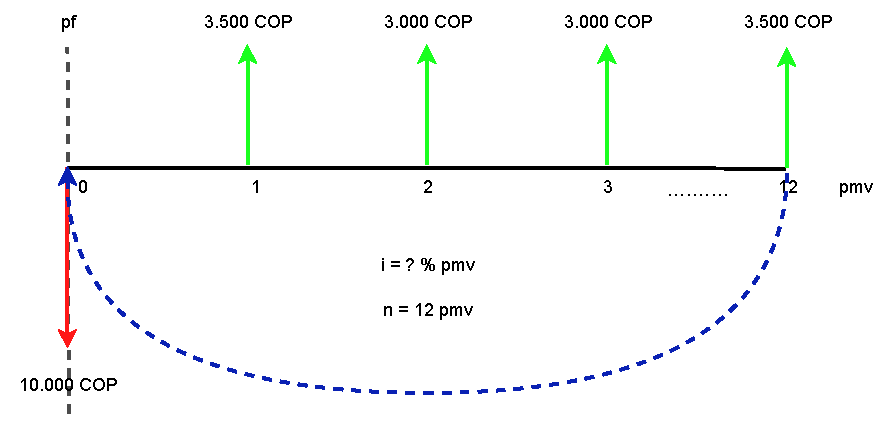
\includegraphics[scale=0.8]{ejemplos/5/Graf2Ej5Cap11.pdf} }
		\\
		\multicolumn{3}{|c|}{$ VPN(B-C)= -  10\text{.}000\text{ } COP +   3\text{.}500(1+i)^{-1}\text{ } COP + 3\text{.}000(1+i)^{-2}\text{ } COP  + $}
		\\
		\multicolumn{3}{|c|}{$  3\text{.}000(1+i)^{-3}\text{ } COP + 3\text{.}500(1+i)^{-4}\text{ } COP =   $ 0 $\text{ } COP$}
		\\
		\multicolumn{3}{|c|}{$ \text{TIRI = 11,41\% pmv, lo cual nos indica que el excedente de inversión (10.000 COP)} $}
		\\
		\multicolumn{3}{|c|}{$ \text{genera un interés del 1,41\% pmv que es inferior a la TMAR,}$}
		\\
		\multicolumn{3}{|c|}{$\text{ en consecuencia, el proyecto más costoso no es aconsejable por} $}
		\\
		\multicolumn{3}{|c|}{$ \text{ lo tanto nos quedamos con el proyecto C.} $}
		\\
		\multicolumn{3}{|c|}{$ \textbf{Se concluye así, que si B > A y C > B entonces C > B > A } $}
		\\
		\multicolumn{3}{|c|}{$ \textbf{ por lo tanto la decisión final es invertir en el proyecto C.} $}                    \\  \hline
		\multicolumn{3}{|c|}{$\text{Comprobación de la decisión usando el VPN usando la TMAR.}$}
		\\
		\multicolumn{3}{|c|}{$VPN(B)= $}
		\\
		\multicolumn{3}{|c|}{$ -  120\text{.}000\text{ } COP -  2\text{.}000(1+0.025)^{-1}\text{ } COP -  3\text{.}000(1+0.25)^{-2}\text{ } COP - $}
		\\
		\multicolumn{3}{|c|}{$ 4\text{.}000(1+0.25)^{-3}\text{ } COP - 5\text{.}000(1+0.25)^{-4}\text{ } COP$}
		\\
		\multicolumn{3}{|c|}{$ VPN(B)= -  127\text{.}616\text{ } COP $}
		\\
		\multicolumn{3}{|c|}{$ VPN(C)=  $}
		\\
		\multicolumn{3}{|c|}{$ -  110\text{.}000\text{ } COP - 5\text{.}500(1+0.025)^{-1}\text{ } COP - 6\text{.}000(1+0.25)^{-2}\text{ } COP - $}
		\\
		\multicolumn{3}{|c|}{$ 7\text{.}000(1+0.25)^{-3}\text{ } COP - 8\text{.}500(1+0.25)^{-4}\text{ } COP $}
		\\
		\multicolumn{3}{|c|}{$ VPN(C)=-  $ $ 125\text{.}306\text{ } COP $}
		\\
		\hline

		%%%%%%%%%% FIN MATEMÁTICAS
		%%%%%% FIN DESARROLLO MATEMÁTICO
		%%%%%% INICIO RESPUESTA
		\rowcolor[HTML]{FFB183}
		%%%%%%%%%%INICIO TITULO
		\multicolumn{3}{|c|}{\cellcolor[HTML]{FFB183}\textbf{6. Respuesta}}                                                 \\ \hline
		%%%%%%%%%% FIN TITULO
		%%%%%%%%%% INICIO RESPUESTA MATEMÁTICA

		\multicolumn{3}{|c|}{ \text{La mejor alternativa es el proyecto C,esto se puede comprobar porque el VPN de este proyecto}}
		\\
		\multicolumn{3}{|c|}{\text{es el mayor, la decisión es coincidente con la que indica la TIRI. } }
		\\
		\hline


		%%%%%%%%%% FIN MATEMÁTICAS
		%%%%%% FIN RESPUESTA
	\end{longtable}
	%Se crean dos lineas en blanco para que no quede el siguiente texto tan pegado
	%\newline \newline %USARLO SI CREES QUE ES NECESARIO
\end{center}
%%%%%%%%%%%%%%%%%%%%%%%%%%FIN EJERCICIO 1 %%%%%%%%%%%%%%%%%%%%%%%%%%%


\newpage
\textbf{Ejemplo 6}\\
Una persona dispone de 6.000.000 COP y como primera alternativa los puede invertir en la alternativa A que le paga un interés del 33\% nominal anual año vencido, pero solo acepta como mínimo la suma de  5.000.000 COP a un año. Como segunda alternativa puede comprar una máquina a un costo de  4.000.000 COP que le producirá ingresos mensuales por valor de  200.000 COP y al final del año podrá vender la máquina en  3.000.000 COP. Los dineros que genere la máquina podrán ser reinvertidos en la alternativa B que recibe cualquier cantidad de dinero y por cualquier tiempo siempre que no sea inferior a un mes, pero solo paga el 2\% periodo mes vencido. ¿Cuál de las dos alternativas debe tomar?
\\


\textbf{Solución.}\\

%La tabla ira centrada
\begin{center}
	\renewcommand{\arraystretch}{1.5}% Margenes de las celdas
	%Creación de la cuadricula de 3 columnas
	\begin{longtable}[H]{|c|c|c|}
		%Creamos una linea horizontal
		\hline
		%Definimos el color de la primera fila
		\rowcolor[HTML]{FFB183}
		%%%%% INICIO ASIGNACIÓN PERÍODO FOCAL %%%%%%%
		%%%%%%%%%% INICIO TITULO
		%Lo que se hace aquí es mezclar las 3 columnas en una sola
		\multicolumn{3}{|c|}{\cellcolor[HTML]{FFB183}\textbf{1. Asignación período focal}}                                                                                                                                                                                             \\ \hline
		%%%%%%%%%% FIN TITULO
		%%%%% INICIO DECLARACIÓN DE VARIABLES %%%%%%%
		\multicolumn{3}{|c|}{$pf : 0 pmv$}                                                                                                                                                                                                                                             \\ \hline

		%%%%%%%%%%% INICIO TITULO
		\rowcolor[HTML]{FFB183}
		\multicolumn{3}{|c|}{\cellcolor[HTML]{FFB183}\textbf{2. Declaración de variables}}                                                                                                                                                                                             \\ \hline
		\multicolumn{1}{|c|}{\cellcolor[HTML]{FFB183}\phantom{000}\textbf{Valores monetarios}\phantom{000}} & \multicolumn{1}{c|}{\cellcolor[HTML]{FFB183}\phantom{000}\textbf{Valores no monetarios}\phantom{000}} & \multicolumn{1}{c|}{\cellcolor[HTML]{FFB183}\textbf{Incógnitas}} \\ \hline
		%%%%%%%%%%% FIN TITULO
		%%%%%%%%%%% INICIO MATEMÁTICAS

		$ Alternativa\text{ } A $                                                                           & $ Alternativa\text{ } A  $                                                                            & $ Alternativa\text{ } A  $                                       \\
		$ P =  6\text{.}000\text{.}000\text{ } COP $                                                        & $J_x$ $=33\% naav $                                                                                   & $F_A = ?\text{ } COP$                                            \\
		$ Alternativa\text{ } B $                                                                           & $ Alternativa\text{ } B  $                                                                            & $ Alternativa\text{ } B  $                                       \\
		$ P = 4\text{.}000\text{.}000\text{ }\text{ } COP  $                                                & $ i_y = 2\%\text{ } pmv $                                                                             & $F_B = ?\text{ } COP$                                            \\
		$ F = 3\text{.}000\text{.}000\text{ }\text{ } COP $                                                 &                                                                                                       &                                                                  \\
		\hline
		%%%%%%%%%% FIN MATEMÁTICAS

		%%%%% INICIO FLUJO DE CAJA
		\rowcolor[HTML]{FFB183}
		\multicolumn{3}{|c|}{\cellcolor[HTML]{FFB183}\textbf{3. Diagrama de flujo de caja}}                                                                                                                                                                                            \\ \hline
		\multicolumn{3}{|c|}{$ $}
		%Mezclamos 3 columnas y pondremos el dibujo
		%%%%%%%%%%%%% INSERCIÓN DE LA IMAGEN
		%Deberán descargar las imágenes respectivas del drive y pegarlas en la carpeta
		%n_capitulo/img/ejemplos/1/capitulo1ejemplo1.pdf  (el /1/ es el numero del ejemplo)
		\\
		\multicolumn{3}{|c|}{$ \text{Alternativa A} $}
		\\

		\multicolumn{3}{|c|}{ 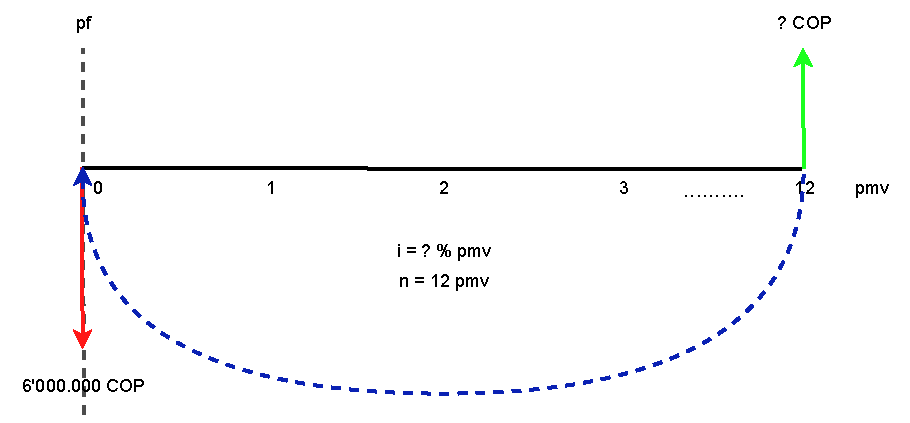
\includegraphics[scale=0.8]{ejemplos/6/Graf1Ej6Cap11.pdf} }                                                                                                                                                                                              \\
		\multicolumn{3}{|c|}{$ $}                                                                                                                                                                                                                                                      \\
		\hline
		\newpage
		\multicolumn{3}{|c|}{$ \text{Alternativa B} $}
		\\
		\multicolumn{3}{|c|}{$ $}                                                                                                                                                                                                                                                      \\
		\multicolumn{3}{|c|}{ 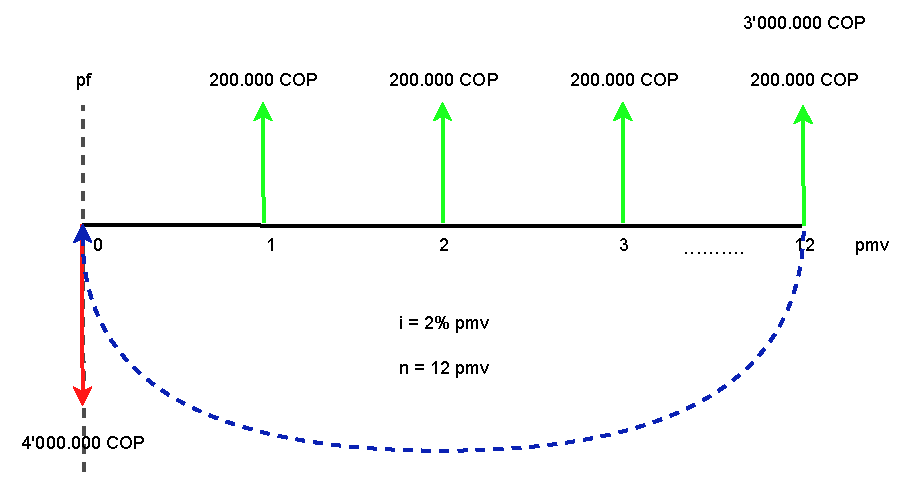
\includegraphics[scale=0.8]{ejemplos/6/Graf2Ej6Cap11.pdf} }                                                                                                                                                                                              \\
		\multicolumn{3}{|c|}{$ $}
		\\
		\multicolumn{3}{|c|}{$ \text{Reinversión} $}
		\\
		\multicolumn{3}{|c|}{$ $}                                                                                                                                                                                                                                                      \\
		\multicolumn{3}{|c|}{ 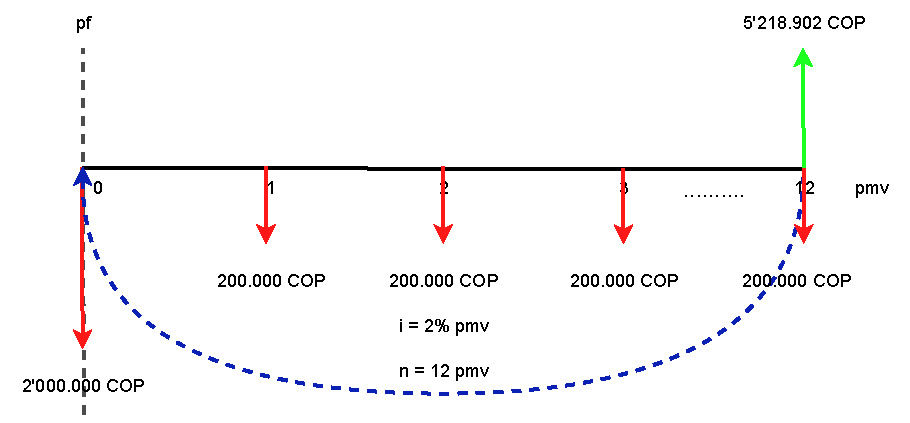
\includegraphics[scale=0.8]{ejemplos/6/Graf3Ej6Cap11.pdf} }

		\\\hline
		%%%%%%%%%%%%% FIN INSERCIÓN DE IMAGEN
		%%%%%FIN FLUJO DE CAJA



		%%%%% INICIO DECLARACIÓN FORMULAS
		%%%%%%%%%%% INICIO TITULO
		\rowcolor[HTML]{FFB183}
		\multicolumn{3}{|c|}{\cellcolor[HTML]{FFB183}\textbf{4. Declaración de fórmulas}}                                                                                                                                                                                              \\ \hline
		%%%%%%%%%%% FIN TITULO
		%%%%%%%%%%% INICIO MATEMÁTICAS
		\multicolumn{3}{|c|} {VPN =	$\sum F_{n}(1+i)^{-n}$   Valor presente neto.}                                                                                                                                                                                                     \\ \hline

		%%%%%%%%%% FIN MATEMÁTICAS
		%%%%%% INICIO DESARROLLO MATEMÁTICO
		\rowcolor[HTML]{FFB183}
		%%%%%%%%%%INICIO TITULO
		\multicolumn{3}{|c|}{\cellcolor[HTML]{FFB183}\textbf{5. Desarrollo matemático}}                                                                                                                                                                                                \\ \hline
		%%%%%%%%%% FIN TITULO
		%%%%%%%%%% INICIO MATEMÁTICAS
		\multicolumn{3}{|c|}{$ \text{La alternativa A le produce el 33\% naav} $}
		\\

		\multicolumn{3}{|c|}{$ \text{sobre el total de su capital ( 6'000.000  COP )} $}
		\\
		\multicolumn{3}{|c|}{$ \text{mientras que en la segunda alternativa podrá comprar la máquina}$}
		\\
		\multicolumn{3}{|c|}{$ \text{y le sobrarán   2'000.000  COP que podrá invertir en la alternativa B.}$}
		\\
		\multicolumn{3}{|c|}{$ \text{Y, además cada vez que la máquina le produzca un ingreso podrá} $}
		\\
		\multicolumn{3}{|c|}{$ \text{ser reinvertido en la alternativa B. Esta segunda} $}
		\\
		\multicolumn{3}{|c|}{$ \text{alternativa podría considerarse como formada por dos proyectos} $}
		\\
		\multicolumn{3}{|c|}{$ \text{así:} $}
		\\
		\multicolumn{3}{|c|}{$   2\text{.}000\text{.}000(1+0.02)^{12}\text{ } COP +   2\text{.}000\text{.}000(1+0.02)^{12}\text{ } COP ..... =    5\text{.}218\text{.}902\text{ } COP $}
		\\
		\multicolumn{3}{|c|}{$ \text{Al fusionar el primero y el segundo proyecto en uno solo se} $}
		\\
		\multicolumn{3}{|c|}{$\text{obtiene un tercer proyecto con egresos de  6'000.000  COP }$}
		\\
		\multicolumn{3}{|c|}{$\text{(   4'000.000  COP +    2'000.000  COP) y con ingresos de    8'218.902  COP}$}
		\\
		\multicolumn{3}{|c|}{$ \text{que resultan de la suma de    3'000.000  COP +  COP  5'218.902 COP} $}
		\\
		\multicolumn{3}{|c|}{$ $}
		\\
		\multicolumn{3}{|c|}{ 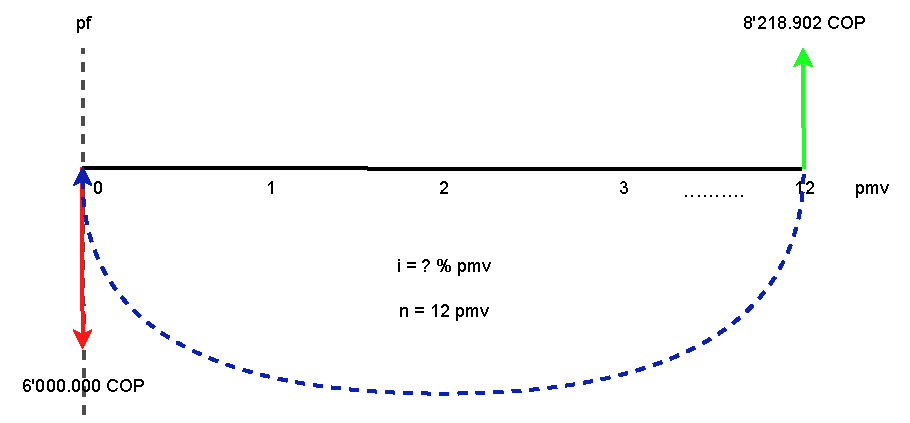
\includegraphics[scale=0.8]{ejemplos/6/Graf4Ej6Cap11.pdf} }
		\\
		\multicolumn{3}{|c|}{$ $}
		\\

		\multicolumn{3}{|c|}{$ \text{A este tercer proyecto se le puede calcular una tasa la cual}$}
		\\
		\multicolumn{3}{|c|}{$\text{viene a ser TIR+R puesto que incluye reinversión y solo usamos}$}
		\\
		\multicolumn{3}{|c|}{$\text{una tasa que es la de reinversión.}$}
		\\
		\multicolumn{3}{|c|}{$\text{La tasa de este último proyecto la calcularemos anual para }$}
		\\
		\multicolumn{3}{|c|}{$\text{compararla con la primera alternativa. }$}
		\\
		\multicolumn{3}{|c|}{$   8\text{'}218\text{.}902\text{ }\text{ } COP =   6\text{'}000\text{.}000(1 + i)^{1}\text{ } COP$}
		\\
		\hline

		%%%%%%%%%% FIN MATEMÁTICAS
		%%%%%% FIN DESARROLLO MATEMÁTICO
		%%%%%% INICIO RESPUESTA
		\rowcolor[HTML]{FFB183}
		%%%%%%%%%%INICIO TITULO
		\multicolumn{3}{|c|}{\cellcolor[HTML]{FFB183}\textbf{6. Respuesta}}                                                                                                                                                                                                            \\ \hline
		%%%%%%%%%% FIN TITULO
		%%%%%%%%%% INICIO RESPUESTA MATEMÁTICA

		\multicolumn{3}{|c|}{ \text{Se escoge la alternativa B, puesto que esta genera una rentabilidad del 36,98\% naav, mientras  }}
		\\
		\multicolumn{3}{|c|}{\text{que la primera solo genera el 33\% naav. } }
		\\
		\hline


		%%%%%%%%%% FIN MATEMÁTICAS
		%%%%%% FIN RESPUESTA
	\end{longtable}
	%Se crean dos lineas en blanco para que no quede el siguiente texto tan pegado
	%\newline \newline %USARLO SI CREES QUE ES NECESARIO
\end{center}
%%%%%%%%%%%%%%%%%%%%%%%%%%FIN EJERCICIO 1 %%%%%%%%%%%%%%%%%%%%%%%%%%%

\textbf{Ejemplo 7}\\
Una industria puede adquirir una máquina a un costo de 6.000.000 COP, tendrá una vida útil de 5 años y prácticamente no tendrá valor de salvamento, la máquina será totalmente depreciada en 3 años por partes iguales, el estudio de mercados indica que los ingresos del primer año serán aproximadamente de 3.000.000 COP y aumentarán todos los años un 30\% periodo año vencido, por otra parte, se estima que el costo de producción del primer año será de 800.000 COP y cada año aumentará en 200.000 COP. Suponiendo una tasa impositiva del 38\% nominal anual año vencido. Determinar la rentabilidad del proyecto usando un horizonte de planeación de 5 años.
\\
\newpage
\textbf{Solución.}\\
%La tabla ira centrada
\begin{center}
	\renewcommand{\arraystretch}{1.5}% Margenes de las celdas
	%Creación de la cuadricula de 3 columnas
	\begin{longtable}[H]{|c|c|c|}
		%Creamos una linea horizontal
		\hline
		%Definimos el color de la primera fila
		\rowcolor[HTML]{FFB183}
		%%%%% INICIO ASIGNACIÓN PERÍODO FOCAL %%%%%%%
		%%%%%%%%%% INICIO TITULO
		%Lo que se hace aquí es mezclar las 3 columnas en una sola
		\multicolumn{3}{|c|}{\cellcolor[HTML]{FFB183}\textbf{1. Asignación período focal}}                                                                                                                                                                                             \\ \hline
		%%%%%%%%%% FIN TITULO
		%%%%% INICIO DECLARACIÓN DE VARIABLES %%%%%%%
		\multicolumn{3}{|c|}{$pf : 0pav$}                                                                                                                                                                                                                                              \\ \hline

		%%%%%%%%%%% INICIO TITULO
		\rowcolor[HTML]{FFB183}
		\multicolumn{3}{|c|}{\cellcolor[HTML]{FFB183}\textbf{2. Declaración de variables}}                                                                                                                                                                                             \\ \hline
		\multicolumn{1}{|c|}{\cellcolor[HTML]{FFB183}\phantom{000}\textbf{Valores monetarios}\phantom{000}} & \multicolumn{1}{c|}{\cellcolor[HTML]{FFB183}\phantom{000}\textbf{Valores no monetarios}\phantom{000}} & \multicolumn{1}{c|}{\cellcolor[HTML]{FFB183}\textbf{Incógnitas}} \\ \hline
		%%%%%%%%%%% FIN TITULO
		%%%%%%%%%%% INICIO MATEMÁTICAS
		$ P_{1} = 6\text{.}000\text{.}000 \text{ COP}$                                                      & $i_{1} = 30\% pav$                                                                                    & $ FNC = ? $                                                      \\
		$\textbf{Ingresos primer año}: 3\text{.}000\text{.}000\text{ COP}$                                  & $\textbf{Tasa impositiva}: i = 38\% pav$                                                              & $VPN = ?\text{ COP}$                                             \\
		$\textbf{Costo primer año}: 800\text{.}000\text{ COP}$                                              & $n = 5 pav$                                                                                           & $i_{R} = ? pav$                                                  \\
		$\textbf{Aumento coste por año}: 200\text{.}000\text{ COP}$                                         &                                                                                                       &                                                                  \\
		\hline
		%%%INICIO DIAGRAMA DE FLUJO
		%%INICIO TITULO
		\multicolumn{3}{|c|}{\cellcolor[HTML]{FFB183}\textbf{3. Diagrama de flujo de caja}}                                                                                                                                                                                            \\ \hline
		%%FIN TITULO
		%%%%%%%%%%%%% INSERCIÓN DE LA IMAGEN
		%Mezclamos 3 columnas y pondremos el dibujo
		%Deberán descargar las imágenes respectivas del drive y pegarlas en la carpeta
		%n_capitulo/img/ejemplos/1/capitulo1ejemplo1.pdf  (el /1/ es el numero del ejemplo)
		\multicolumn{3}{|c|}{ 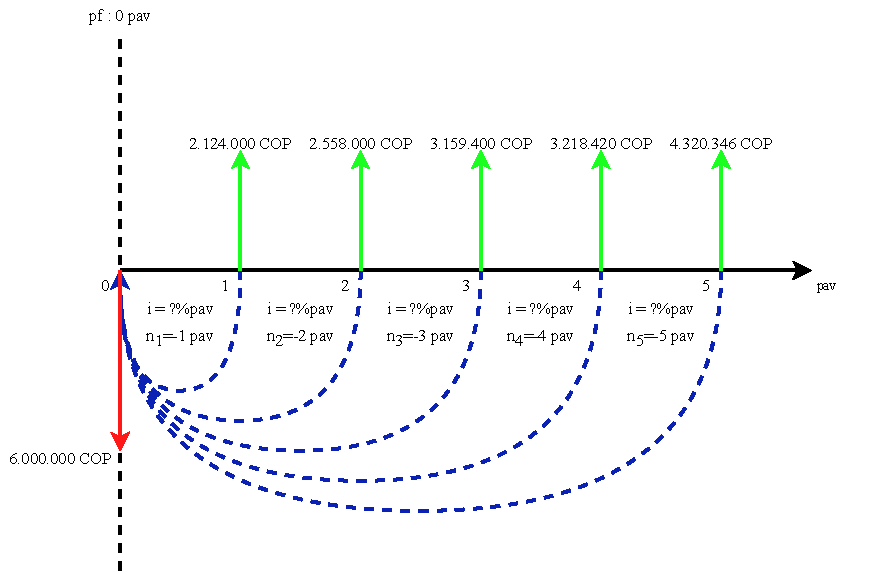
\includegraphics[scale=0.8]{ejemplos/7/Graf1Ej7Cap11.pdf} }
		\\ \hline
		%%%%%%%%%%%%% FIN INSERCIÓN DE IMAGEN
		%%%FIN DIAGRAMA DE FLUJO



		%%%%% INICIO DECLARACIÓN FORMULAS
		%%%%%%%%%%% INICIO TITULO
		\rowcolor[HTML]{FFB183}
		\multicolumn{3}{|c|}{\cellcolor[HTML]{FFB183}\textbf{4. Declaración de fórmulas}}                                                                                                                                                                                              \\ \hline
		%%%%%%%%%%% FIN TITULO
		%%%%%%%%%%% INICIO MATEMÁTICAS
		\multicolumn{3}{|c|} {$ \text{Base = Ingreso — Costo — Depreciación.} $}                                                                                                                                                                                                       \\
		\multicolumn{3}{|c|} {$ \text{Impuesto = Tasa impositiva x Base} $}                                                                                                                                                                                                            \\
		\multicolumn{3}{|c|} {$ \textbf{Flujo Neto de Caja: } \text{FNC = Ingreso — Costo — Impuesto } $}                                                                                                                                                                              \\
		\multicolumn{3}{|c|} {$VPN =\sum F_{n}(1+i)^{-n} $ Valor presente neto.}                                                                                                                                                                                                       \\
		\hline

		%%%%%%%%%% FIN MATEMÁTICAS
		%%%%%% INICIO DESARROLLO MATEMÁTICO
		\rowcolor[HTML]{FFB183}
		%%%%%%%%%%INICIO TITULO
		\multicolumn{3}{|c|}{\cellcolor[HTML]{FFB183}\textbf{5. Desarrollo matemático}}                                                                                                                                                                                                \\ \hline
		%%%%%%%%%% FIN TITULO
		%%%%%%%%%% INICIO MATEMÁTICAS
		\multicolumn{3}{|c|}{$ \text{A continuación presentamos la tabla necesaria para calcular el flujo de caja.} $}
		\\
		%%\multicolumn{3}{|c|}{ \includegraphics[scale=0.7]{7/Graf2Ej7Cap11.pdf} }   
		\multicolumn{3}{|c|}{ }
		\\
		\multicolumn{3}{|c|}{}                                                                                                                                                                                                                                                         \\
		\multicolumn{3}{|c|}{
			{\fontsize{8.5}{10}\selectfont
					\begin{tabular}{|>{\centering\arraybackslash}p{0.3cm}|>{\centering\arraybackslash}p{1.8cm}|>{\centering\arraybackslash}p{1.9cm}|>{\centering\arraybackslash}p{1.8cm}|>{\centering\arraybackslash}p{1.9cm}|>{\centering\arraybackslash}p{1.9cm}|>{\centering\arraybackslash}p{1.9cm}|}
						\hline
						\rowcolor{white!50}
						\textbf{Per} & \textbf{Ingreso}                   & \textbf{Costo}                     & \textbf{Depreciación}              & \textbf{Base}                      & \textbf{Impuesto}                  & \textbf{FNC}                       \\ \hline
						\text{0}     & \text{6\text{.}000\text{.}000 COP} & \text{0 COP}                       & \text{0 COP}                       & \text{0 COP}                       & \text{0 COP}                       & \text{6\text{.}000\text{.}000 COP} \\ \hline
						\text{1}     & \text{3\text{.}000\text{.}000 COP} & \text{800\text{.}000 COP}          & \text{2\text{.}000\text{.}000 COP} & \text{200\text{.}000 COP}          & \text{76\text{.}000 COP}           & \text{2\text{.}124\text{.}000 COP} \\ \hline
						\text{2}     & \text{3\text{.}900\text{.}000 COP} & \text{1\text{.}000\text{.}000 COP} & \text{2\text{.}000\text{.}000 COP} & \text{900\text{.}000 COP}          & \text{342\text{.}000 COP}          & \text{2\text{.}558\text{.}000 COP} \\ \hline
						\text{3}     & \text{5\text{.}070\text{.}000 COP} & \text{1\text{.}200\text{.}000 COP} & \text{2\text{.}000\text{.}000 COP} & \text{1\text{.}870\text{.}000 COP} & \text{710\text{.}000 COP}          & \text{3\text{.}159\text{.}400 COP} \\ \hline
						\text{4}     & \text{6\text{.}591\text{.}000 COP} & \text{1\text{.}400\text{.}000 COP} & \text{-}                           & \text{5\text{.}191\text{.}000 COP} & \text{1\text{.}972\text{.}000 COP} & \text{3\text{.}218\text{.}420 COP} \\ \hline
						\text{5}     & \text{8\text{.}568\text{.}300 COP} & \text{1\text{.}600\text{.}000 COP} & \text{-}                           & \text{6\text{.}968\text{.}000 COP} & \text{2\text{.}647\text{.}954 COP} & \text{4\text{.}320\text{.}346 COP} \\ \hline
					\end{tabular}
				}
		}                                                                                                                                                                                                                                                                              \\
		\multicolumn{3}{|c|}{ }                                                                                                                                                                                                                                                        \\
		\multicolumn{3}{|c|}{$ \text{Si hacemos el VPN = 0 podemos hallar la TIR.} $}
		\\
		\multicolumn{3}{|c|}{$VPN = -6\text{.}000\text{.}000 COP +  2\text{.}124\text{.}000 COP(1+i)^{-1} +  2\text{.}558\text{.}000 COP(1+i)^{-2} $}
		\\
		\multicolumn{3}{|c|}{$ +3\text{.}159\text{.}400 COP(1+i)^{-3} + 3\text{.}218\text{.}420 COP(1+i)^{-4} +  4\text{.}320\text{.}346 COP(1+i)^{-5} = 0 \text{ COP}$}
		\\
		\multicolumn{3}{|c|}{$ \text{Al resolver esta ecuación por interpolación se obtiene:} $}
		\\
		\multicolumn{3}{|c|}{$ \text{i = 36,58\% pav} $}
		\\
		\hline

		%%%%%%%%%% FIN MATEMÁTICAS
		%%%%%% FIN DESARROLLO MATEMÁTICO
		%%%%%% INICIO RESPUESTA
		\rowcolor[HTML]{FFB183}
		%%%%%%%%%%INICIO TITULO
		\multicolumn{3}{|c|}{\cellcolor[HTML]{FFB183}\textbf{6. Respuesta}}                                                                                                                                                                                                            \\ \hline
		%%%%%%%%%% FIN TITULO
		%%%%%%%%%% INICIO RESPUESTA MATEMÁTICA

		\multicolumn{3}{|c|}{ $\text{La rentabilidad del proyecto es del 36,58\% pav}$}
		\\
		\hline


		%%%%%%%%%% FIN MATEMÁTICAS
		%%%%%% FIN RESPUESTA
	\end{longtable}
	%Se crean dos lineas en blanco para que no quede el siguiente texto tan pegado
	%\newline \newline %USARLO SI CREES QUE ES NECESARIO
\end{center}
%%%%%%%%%%%%%%%%%%%%%%%%%%FIN EJERCICIO 1 %%%%%%%%%%%%%%%%%%%%%%%%%%%

